\section{Entwurf einer Besiedlungsgeschichte für das Kongobecken}\label{sec:Zeitscheiben}	

Der aus der Zusammenschau der diskutierten regionalen Sequenzen entwickelte Entwurf eines Chronologieschemas für das Kongobecken (Abb.~\ref{fig:Chronologiesystem}) reflektiert eine Reihe kulturhistorischer Entwicklungen, die im Folgenden diskutiert werden sollen. Die knapp 2500~Jahre umspannende keramische Entwicklungsgeschichte der Region wird dafür in drei Perioden unterteilt: eine vom Beginn der Besiedlung im 4.~Jh.~v.~Chr. bis in das 6.~Jh.~n.~Chr. reichende Frühen Eisenzeit, eine vom 7.--11.~Jh.~n.~Chr. datierende Mittlere Eisenzeit und schließlich die ab dem 12.~Jh.~n.~Chr. bis in die Gegenwart andauernde Späte Eisenzeit. Aus dem untersuchten keramischen Inventar liegen keine dezidierten europäischen Importfunde vor; daher wird eine historische Periode, wie sie beispielsweise in Gabun beobachtet werden kann (Kap.~\ref{sec:Gabun}), nicht abgegrenzt wird. Sie ließe sich potentiell erst mit der Erschließung des Kongobeckens durch die europäischen Kolonialmächte in der zweiten Hälfte des 19.~Jh.~n.~Chr. postulieren. Ein direkter Einfluss auf die Entwicklung der lokalen Töpfereitraditonen kann gegenwärtig jedoch nicht beobachtet werden. Die Frühe wie Späte Eisenzeit können jeweils noch in drei Stufen untergliedert werden. Dieser Entwurf einer Periodisierung ist als eine relative Zeitdifferenzierung anzusehen und liefert vornehmlich eine Diskussionsbasis, um potentiell zeitgleiche Phänomene betrachten zu können. Aussagen im Sinne einer entwicklungsgeschichtlichen Kulturklassifikation lassen sich nicht daraus ableiten \parencite[siehe][40--43]{Eggert.2012e}.\footnote{So lässt sich die \enquote*{Ablösung} von flachbodiger durch rundbodiger Keramik sowie das Aufkommen von Rouletteverzierung nur sehr begrenzt als entwicklungsgeschichtlicher Marker im Sinne einer Kulturklassifikation diskutieren, da es sich lediglich um Eigenschaften der Keramik handelt.}

Eine von \textcite[1379 Tab.~1]{Oslisly.2013b} vorgeschlagene Periodisierung für das westliche Zentralafrika\footnote{Das Arbeitsgebiet der Studie von \textcite[1377]{Oslisly.2013b} liegt zwischen 7$^\circ$~N--6$^\circ$~S sowie 9--20$^\circ$~O und umfasst Daten aus dem Süden Kameruns, dem kontinentalen Äquatorialguinea, Gabun, der Republik Kongo und der westlichen Demokratischen Republik Kongo sowie dem Südwesten der Zentralafrikanischen Republik.} beginnt mit der in der Mitte des 2.~Jt.~v.~Chr. endende \textit{Later Stone Age}, gefolgt  von einer bis in das 1.~Jh.~v.~Chr. andauernden \enquote*{neolithischen} Phase.\footnote{Im Laufe des 1.~Jt.~v.~Chr. folgt die Eisenzeit in weiten Teilen West- und Zentralafrikas direkt und ohne eine dazwischen liegende, dezidierte Kupfer- oder Bronzezeit auf \textit{Later Stone Age}-Komplexe. Aufgrund unsicherer oder fehlender Nachweise für Eisenmetallurgie sowie problembehaftete absolutchronologische Datierungen wird von einigen Autoren eine \textit{neolithische} Phase abgegrenzt \parencites[siehe exemplarisch][]{Clist.2006b}{Oslisly.2006}. Neben dieser augenscheinlich in Anlehnung an europäische Vorbilder vorgebrachten Bezeichnung findet sich auch die Bezeichnung \textit{Stone to Metal Age} \parencites{Maret.19941995}{Lavachery.1996}, die \textcite{McIntosh.1988} für die Situation in Westafrika geprägt haben. Auch werden Parallelen zur für Ostafrika gültigen \textit{Ceramic Later Stone Age} \parencite{Ambrose.1997} gezogen. Jedoch findet sich auch die Nutzung des Konzepts \textit{Neolithikum} nach der ursprünglicheren Definition von \textcite{Lubbock.1865} in der Literatur \parencite[3]{Zangato.2000}. Eine uneingeschränkte Entlehnung aus der europäischen Archäologie für die Situation in Zentralafrika ist jedoch unzulässig, da bislang keine bis kaum stichhaltige Belege für eine produzierende Wirtschaftsweise in den fraglichen Phasen vorliegen. Damit fehlen einem wie auch immer konzeptualisierten \textit{zentralafrikanischem Neolithikum} die sozio-ökonomischen Kritieren \parencite[276f.]{Eggert.2006b}. Diese sind jedoch seit \textcite{Childe.1936} untrennbar mit dem Konzept Neolithikum verbunden. Ein jedes für Zentralafrika postuliertes \textit{Neolithikum} spiegelt folglich lediglich ein auf sekundären Kriterien basierendes archäologisches Konzept wider und beschreibt nicht mehr als die wenig aussagekräftige Assoziation von Keramik und geschliffenen Steinwerkzeugen. Siehe auch die ausführliche Diskussion von \textcite[187f.]{Eggert.2014}. \label{ftn:ZentralafrikaNeolithikum}} Den Beginn der Eisenzeit setzt Oslisly im 8.~Jh.~v.~Chr. an, wobei die von ihm abgegrenzte Periode der Frühen Eisenzeit bis in das 10.~Jh.~n.~Chr. Bestand hat. Die Späte Eisenzeit folgt dann ab dem 11.~Jh.~n.~Chr. \parencite[1379--1381]{Oslisly.2013b}. Die Untersuchung von \textcite{Oslisly.2013b} basiert jedoch auf einer methodisch nicht nachvollziehbaren Zuweisung von -- aufgrund der Kalibration -- über mehrere Jahrhunderte streuenden Radiokohlenstoffdatierungen zu einzelnen, ein Jahrhundert umfassenden Klassen (ebd. 1380 Abb.~3). Auch deckt der für die Analyse herangezogene Datensatz nicht alle verfügbaren Datierungen ab.\footnote{Ein Abgleich der von \textcite{Oslisly.2013b} aufgeführten Datierungen mit dem \textit{Archives des datations radiocarbone d'Afrique centrale} (aDRAC), einer Online-Datenbank der publizierten Radiokohlenstoffdatierungen aus Zentralafrika (\url{https://github.com/dirkseidensticker/aDRAC}; \textsc{Seidensticker} 2016), ergab Abweichungen bei 59 der insgesamt 328 in der Studie einbezogenen Fundstellen. Es sind nahezu alle Fundplätze von denen mehr als 1--2 Datierungen bekannt sind betroffen. Als ein exemplarisches Beispiel soll an dieser Stelle nur auf die Fundstelle Okala in Gabun eingegangen werden. Während die Veröffentlichung von \textcite{Clist.20042005} insgesamt 15 Datierungen aus Okala umfasst, enthält der Datensatz von \textcite{Oslisly.2013b} nur sieben Datierungen. Die nicht enthaltenen Datierungen Beta-20788, Beta-20790 und Beta-25582 sowie Gif-8612, Gif-8966 und Gif-8968 lassen nicht erkennen warum sie von \textcite{Oslisly.2013b} nicht aufgenommen wurden. Lediglich für die Datierung Beta-46142 könnte angeführt werden, das sie aussortiert wurde da sie ein Alter vom 43.--41. Jt.~v.~Chr. ergab, was deutlich außerhalb der durch den Aufsatz betrachteten Zeitspanne liegt. Auch die in die zweite Hälfte des 4.~Jt.~v.~Chr. datierende Probe Gif-8614 fällt aus dem betrachteten Bereich heraus. Die übrigen genannten Daten decken einen Zeitraum vom 7.~Jh.~v.~Chr. bis 4.~Jh.~n.~Chr. ab. Ihr Fehlen in dem der Studie zugrundeliegenden Datensatz lässt sich nicht erklären. \textcite[1378]{Oslisly.2013b} verweisen zwar darauf, dass 94 Datierungen, die sehr ähnliche Ergebnisse lieferten und von jeweils gleichen Fundstellen stammen, aussortiert wurden, jedoch lassen sich die Einzelfälle nicht abprüfen. Dies unterstreicht, wie groß die Abhängigkeit entsprechender, auf Radiokohlenstoffdatierungen basierender Metastudien von der Datenbasis ist.} In ihrer Studie stellen \textcite[1380]{Oslisly.2013b} vor allem einen als Besiedlungshiatus bewerteten Rückgang vorhandener Datierungen im 7./8.--11./12.~Jh.~n.~Chr. vor. Dieser wurde bereits früher von \textcites[101--103~Abb.~9]{Oslisly.1998}[112f.~Abb.~7.9]{Oslisly.2001d} diskutiert.

Die folgende Betrachtung des Besiedlungsgangs gründet auf den Erkenntnissen aus dem vom \textcite{Wotzka.1995} aufgearbeiteten Inventaren aus dem Inneren Kongobecken, ersten Erkenntnissen aus dem nordöstlichen Kongobecken \parencite{LivingstoneSmith.2017} sowie den in der vorliegenden Arbeit gewonnen Erkenntnissen zum nordwestlichen Kongobecken.\footnote{Die Kartierungen (Abb.~\ref{fig:EIA1_Karte}--\ref{fig:LIA3_Karte}) decken das Kongobecken zwischen 6$^\circ$~Nord und 2$^\circ$~Süd sowie 15$^\circ$~Ost bis 26$^\circ$~Ost an. Es wurden nur solche Fundstellen kartiert an denen eine spezifische Stilgruppe sicher nachgewiesen wurde. Fundstellen aus dem Arbeitsgebiet, an denen eine Stilgruppe nur unter Vorbehalt nachgewiesen wurde sind in den Verbreitungskarten in Kap.~\ref{sec:Keramiksequenz} verzeichnet.}

\begin{figure*}[p]
	\centering
	\begin{subfigure}[b]{\textwidth}
		\centering
		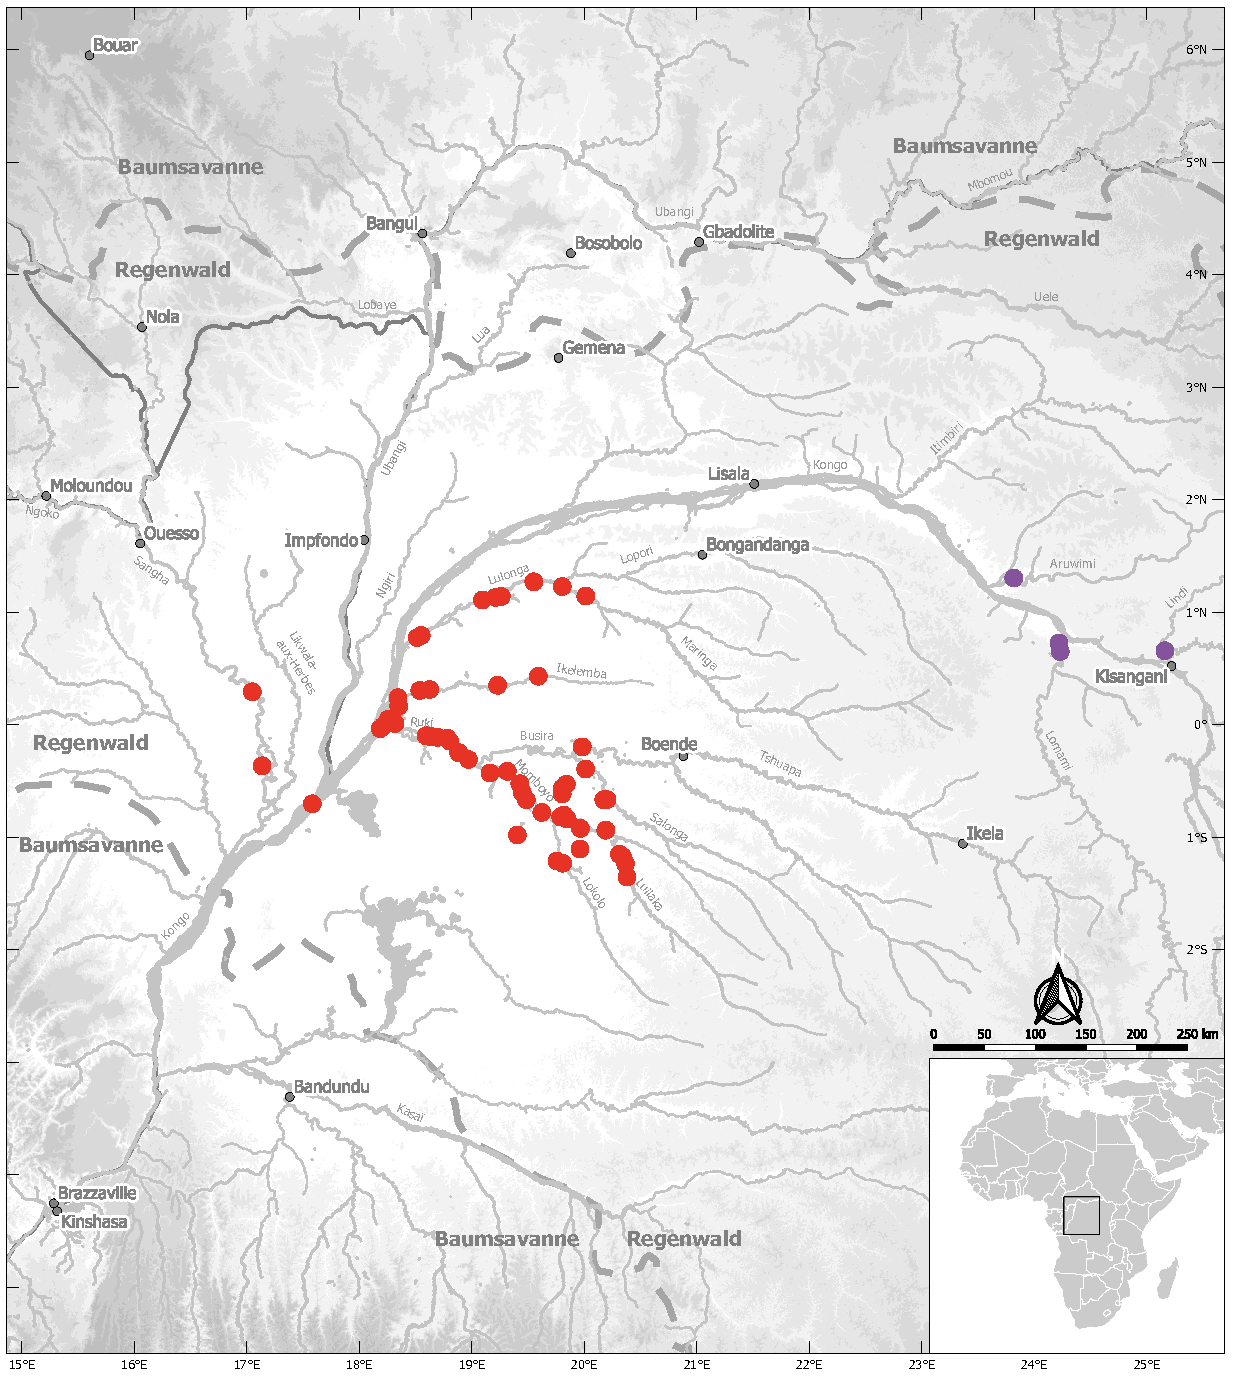
\includegraphics[width = \textwidth]{GIS/output/5-7_Zeitscheibe_EIA1_A4print-2.pdf}
		\vspace{2cm}
		\caption{Verbreitung}
		\label{fig:EIA1_Karte}
	\end{subfigure}
	\caption{Ältere Phase der Frühe Eisenzeit (4.--2. Jh. v. Chr.).}
	\label{}
\end{figure*}
\addtocounter{figure}{-1}
\begin{figure*}[p]
	\begin{subfigure}[b]{\textwidth}
		\setcounter{subfigure}{1}
		\centering
		\includegraphics[width = \textwidth]{figs/Chronologiesystem_v3a_Zeitschiebe_EIA1.pdf}
		\caption{Chronologie}
		\label{fig:EIA1_Chronologie}
	\end{subfigure}
	\caption{Ältere Phase der Frühe Eisenzeit (4.--2. Jh. v. Chr.).}
	\label{fig:EIA1}
\end{figure*}

\subsubsection*{Ältere Phase der Frühen Eisenzeit (4.--2. Jh. v. Chr.)}

Die früheste keramische Entwicklung im Inneren Kongobecken ist durch die Imbonga-Keramik \parencite[59--68]{Wotzka.1995} repräsentiert, die in das 4.--2.~Jh.~v.~Chr. datiert und an 59 Fundstellen beziehungsweise nahezu dem gesamten westlichen Teil des von \textcite{Wotzka.1995} untersuchten Raumes verbreitet ist (Abb.~\ref{fig:EIA1}). Auch im nordöstlichen Kongobecken ist ab dem 4. Jh.~v.~Chr. mit keramischen Zeugnissen zu rechnen. Die an insgesamt vier Fundstellen angetroffene Keramik der ältesten Phase weist auf Basis der vier vorliegenden Radiokohlenstoffdatierungen eine Laufzeit bis mindestens in das 1.~Jh.~n.~Chr. auf \parencite[17 Abb.~23]{LivingstoneSmith.2017}. Zwischen den beiden Gruppen, die nur entfernte formale Ähnlichkeiten zueinander aufweisen (siehe Kap.~\ref{sec:NordCongo}), liegen etwa 400--450\,km, der östliche Teil des von \textcite{Wotzka.1995} untersuchte Raumes, der erst deutlich später aufgesiedelt wurde (Abb.~\ref{fig:LIA1}). Gegenwärtig liegen jedoch keine Erkenntnisse zur Besiedlung entlang des Kongo zwischen der 70\,km nördlich von Mbandaka gelegenen Mündung des Lulonga und den im nordöstlichen Kongobecken liegenden, 2010 erstmals untersuchten Flussläufen vor. Ein verbindendes Element zwischen diesen beiden Stilen, neben der Nutzung ähnlicher Verzierungstechniken wie die in großen Teilen Zentralafrikas verbreitete Wiegebandtechnik, bildet die Beobachtung, dass die frühe Keramik des nordöstlichen Kongobeckens in Aufbautechnik hergestellt ist \parencite[16]{LivingstoneSmith.2017}. Diese Technik lässt sich, aufgrund der geringen Anzahl entsprechend untersuchter Gefäße unter Vorbehalt auch für die Keramik der Imbonga-Gruppe vermuten (Kap.~\ref{sec:Herstellung}; Abb.~\ref{MKA87-102-1_Makrospuren}--\ref{MIT87-103-1_Makrospuren}). Innerhalb der rezenten Töpfereitradition des Inneren Kongobeckens ist die Aufbautechnik das allgemein vorherrschende Herstellungsverfahren (Kap.~\ref{sec:ToepfereiEthnogr}). 

Bestimmendes Kriterium für den Beginn der ältere Phase der Frühe Eisenzeit um 400~v.~Chr. bildet das erste Auftreten von Keramik\footnote{Hinweise auf Eisenmetallurgie in Kontexten der Imbonga-Gruppe ergaben sich bei Grabungen des Kölner Kongoprojektes unter Leitung von H.-P.~Wotzka in Iyonda im Jahr 2015 (mündl. Mitt. Wotzka 2016).\label{ftn:EisenIYO15/2-4}} in Form der Imbonga-Keramik im zentralen Bereich des Kongobeckens sowie die frühe Keramik an seinem nordöstlichen Rand (Abb.~\ref{fig:EIA1}). Gerade durch die in ihrem Verbreitungsgebiet dichten Spuren der Imbonga-Gruppe ist von einer potentiell sehr schnellen ersten Aufsiedlung des westlichen Teils des Inneren Kongobeckens auszugehen.

\subsubsection*{Mittlere Phase der Frühen Eisenzeit (2. Jh. v. Chr. -- 2. Jh. n. Chr.)}

Der Beginn der mittleren Phase der frühen Eisenzeit um 200 v. Chr. wird einerseits durch eine Differenzierung der keramischen Stilentwicklung im Inneren Kongobecken und dem damit verbundenen Ende der Imbonga-Keramik sowie andererseits durch den Beginn einer hinreichend belegbaren Aufsiedlung des nordwestlichen Kongobeckens durch die Pikunda-Munda-Gruppe im Süden (Kap.~\ref{sec:PKM-Gr}) und die Batalimo-Maluba-Gruppe im Norden markiert (Kap.~\ref{sec:BTM-Gr}; Abb.~\ref{fig:EIA2}). Die jüngeren Ausprägungen der Imbonga-Gruppe umfassten nach \textcite{Eggert.1983} noch Merkmale, die von \textcite{Wotzka.1995} in die Stile Bonkake, Ingende und Inganda ausdifferenziert wurden.\footnote{Siehe Anm.~\ref{ftn:AufteilungIMB}.} Eine Ausweitung des Siedlungsareals im Inneren Kongobecken lässt sich nur am unteren Tshuapa, bis in die Region um Boende sowie am unteren Luilaka beobachten. Die keramische Entwicklung in den Jahrhunderten um die Zeitenwende ist vornehmlich von Regionalisierung und Differenzierung geprägt. So ist die Stilgruppe Ingende auf den äußersten Westen des von \textcite{Wotzka.1995} untersuchten Raumes, die Region um Mbandaka beschränkt (ebd. 546f. Karte~3). Auch die Bokele-Gruppe ist nur an zwei Fundorten im Westen des Inneren Kongobeckens nachgewiesen (ebd. 556f. Karte~8). Nur im südlichen Teil des einstiegen Verbreitungsgebietes der Imbonga-Keramik finden sich die Stilgruppen Bonkake (ebd. 546f. Karte~3), Lokondola und Monkoto (ebd. 550f. Karte~5) sowie Lusako (ebd. 552f. Karte~6). Die Yete-Gruppe hat ihren Verbreitungsschwerpunkt im Bereich des Momboyo, findet sich aber ebenfalls ausschließlich im südlichen Teil des Inneren Kongobeckens (ebd. 552f. Karte~6). Lediglich die Inganda-Gruppe kommt nahezu im gesamten, einstigen Verbreitungsgebiet der Imbonga-Gruppe vor (ebd.548f. Karte~4). Im nördlichen Teil des einstigen Verbreitungsgebietes der Imbonga-Gruppe (Abb.~\ref{fig:EIA1_Karte}), entlang des Lulonga ist eher eine Abnahme der Fundstellen zu beobachten. Der Beginn der genannten Stile wird von \textcite{Wotzka.1995} jeweils mit jüngeren Ausprägungen der Imbonga-Keramik in Zusammenhang gebracht und kann daher frühestens in das ausgehende 3. und das 2.~Jh.~v.~Chr. datiert werden.

\begin{figure*}[p]
	\centering
	\begin{subfigure}[b]{\textwidth}
		\centering
		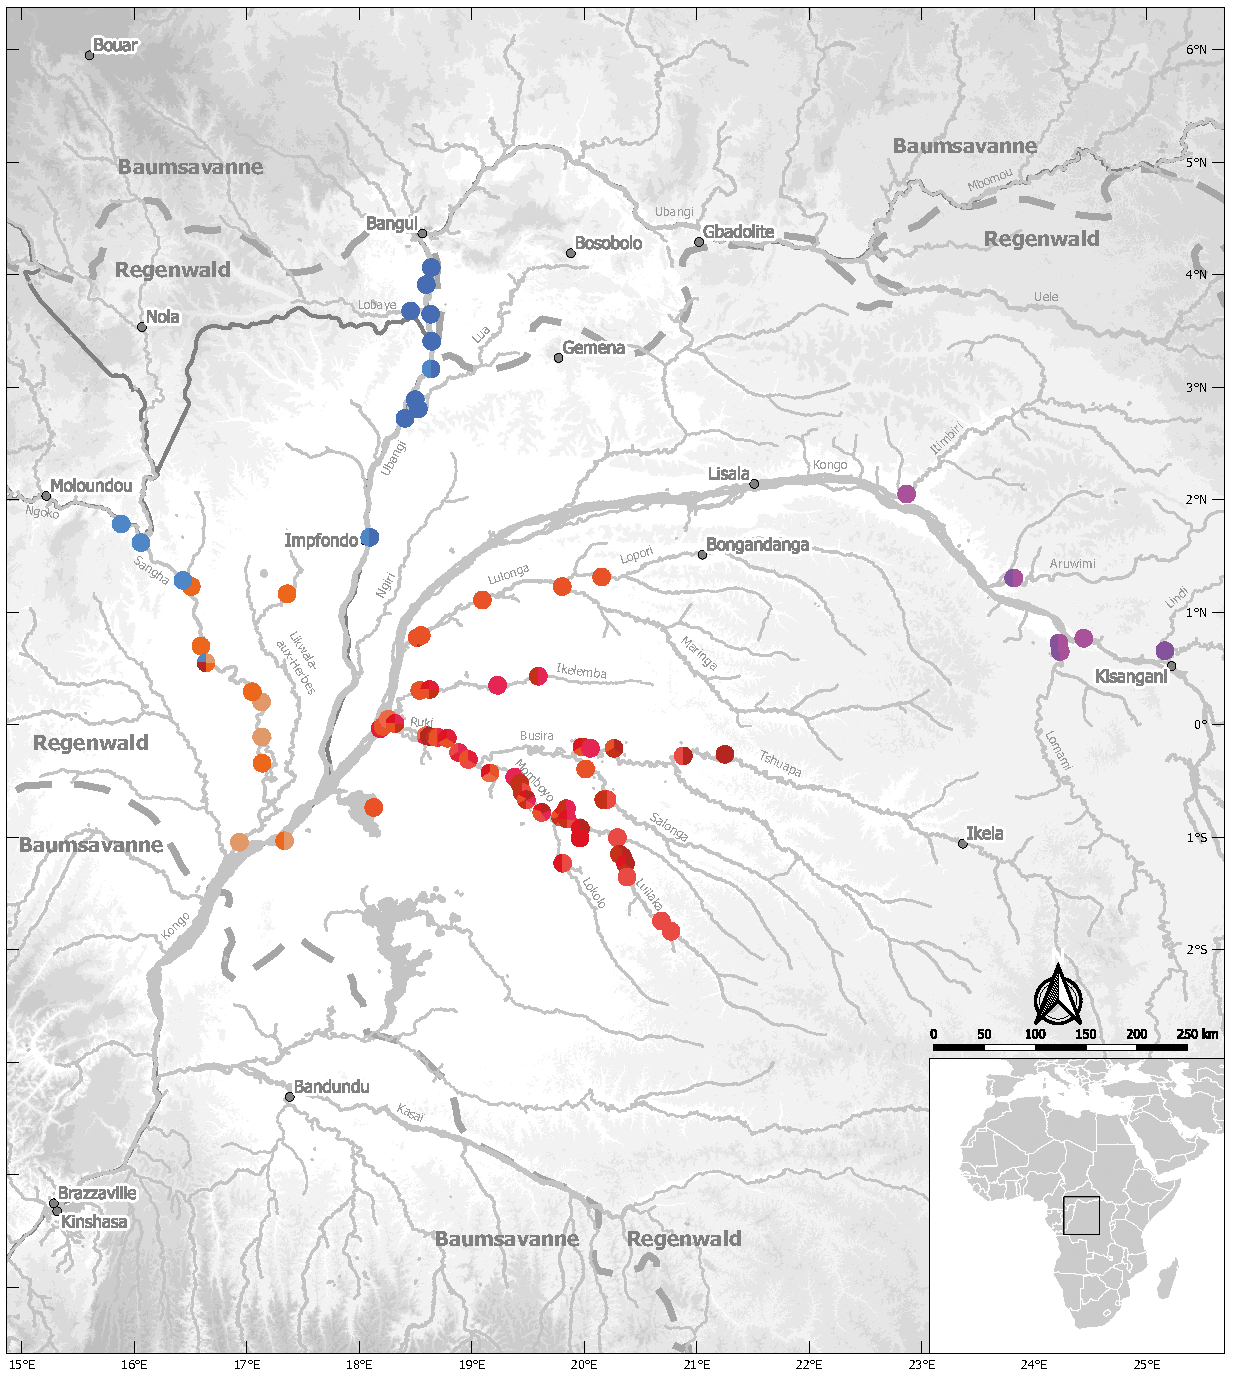
\includegraphics[width = \textwidth]{GIS/output/5-7_Zeitscheibe_EIA2_A4print-2.pdf}
		\vspace{2cm}
		\caption{Verbreitung}
		\label{fig:EIA2_Karte}
	\end{subfigure}
	\caption{Mittlere Phase der Frühe Eisenzeit (2. Jh. v. Chr. -- 2. n. Chr.).}
	\label{}
\end{figure*}
\addtocounter{figure}{-1}
\begin{figure*}[p]
	\begin{subfigure}[b]{\textwidth}
		\setcounter{subfigure}{1}
		\centering
		\includegraphics[width = \textwidth]{figs/Chronologiesystem_v3a_Zeitschiebe_EIA2.pdf}
		\caption{Chronologie}
		\label{fig:EIA2_Chronologie}
	\end{subfigure}
	\caption{Mittlere Phase der Frühe Eisenzeit (2. Jh. v. Chr. -- 2. n. Chr.).}
	\label{fig:EIA2}
\end{figure*}

Im nordwestlichen Kongobecken sind frühestens ab dem 2.~Jh.~v.~Chr. -- in Gestalt der Stile Batalimo-Maluba (Kap.~\ref{sec:BTM-Gr}) und Pikunda-Munda (Kap.~\ref{sec:PKM-Gr}) -- hinreichend umfassende keramische Inventare nachweisbar. Zwar liegen vom Unterlauf des Sangha zwei Nachweise für ältere Imbonga-Keramik vor, jedoch ist einerseits der Kontext dieser Funde unklar und andererseits lassen sich auch in den Surveyfunden anderer Fundstellen keine potentiell der Imbonga-Gruppe zuordenbaren Stücke identifizieren (Kap.~\ref{sec:IMB-Gr}). Die erste eindeutig fassbare Besiedlung des nordwestlichen Kongobeckens durch keramikproduzierende Gruppen erfolgte vielmehr getrennt voneinander, in zwei potentiell auch naturräumlich sich unterscheidenden Regionen. Acht der neun bekannten, sicher Funde der Batalimo-Maluba-Gruppe aufweisenden Fundstellen liegen außerhalb des für die Regenwaldkrise des 1.~Jt.~v.~Chr. von \textcite[7 Abb.~4; Abb.~\ref{fig:Maley2001_7Abb4}]{Maley.2001} postulierten Regenwaldrefugiums. Auch mit Blick auf die heutige Vegetation befinden sich die Fundstellen der Batalimo-Maluba-Gruppe am nördlichen Rand des äquatorialen Regenwaldes. Das es sich bei den Trägern der Batalimo-Maluba-Keramik folglich nicht um Bewohner des Regenwaldes handelte, kann zwar als Hypothese angesehen werden, bedarf aber weiterer Untersuchungen. Das Verbreitungsgebiet der im südlichen Teil des nordwestlichen Kongobeckens, entlang des unteren Sangha sowie des Likwala-aux-Herbes verbreiteten Pikunda-Munda-Keramik liegt heutzutage in ausgedehnten Sumpfwäldern (Abb.~\ref{fig:VegetationKarte}). Alle der mit Pikunda-Munda-Keramik sicher zu assoziierenden Fundstellen liegen innerhalb des von \textcite{Maley.2001} postulierten Regenwaldrefugiums, das hauptsächlich das Innere Kongobecken abdeckt (Abb.~\ref{fig:Maley2001_7Abb4}). Es kann davon ausgegangen werden, dass die die Pikunda-Munda-Keramik tragenden Bevölkerungen, wie auch die zeitgleichen Gruppen im benachbarten Inneren Kongobecken im sich von der Regenwaldkrise des 1.~Jt.~v.~Chr. erholenden äquatorialen Regenwald siedelten \parencite[siehe][337]{Hubau.2013}. Entlang des nordwestlichen Randes des von \textcite{Maley.2001} im Inneren Kongobecken postulierten Regenwaldrefugiums findet sich zeitgleich zu den Stilen Batalimo-Maluba und Pikunda-Munda auch Keramik der Ngbanja-Gruppe (Kap.~\ref{sec:NGB-Gr}). Der tatsächliche ökologische Kontext dieser gegenwärtig nur unter Vorbehalt ansprechbaren Stilgruppe muss jedoch offen bleiben. 

Die Stilgruppen Batalimo-Maluba und Pikunda-Munda weisen kaum formale Gemeinsamkeiten auf und auch in technischer Hinsicht unterscheiden sie sich stark. Dadurch kann gegenwärtig nur von einem getrennten Ursprung dieser beiden Stile ausgegangen werden. Leider lässt sich dieser aus Mangel an entsprechenden Vergleichsfunden von außerhalb des Arbeitsgebietes in beiden Fällen nicht herleiten. Beide Stilgruppen spiegeln deutlich unabhängige keramische Entwicklungen wider.

Im nordöstlichen Kongobecken liegen weiterhin Belege für die Keramik der ältesten Phase vor, die im 1.~Jh.~n.~Chr. durch die formal andersartige Keramik der mittleren Phasen abgelöst wird, die ihrerseits noch bis in das frühe 5.~Jh.~n.~Chr. nachgewiesen ist (Kap.~\ref{sec:NordCongo}; Abb.~\ref{fig:LivingstoneSmith2017_noCongoTrad}.4--7). Die Anwesenheit von Keramik der mittleren Phase in Moenge am unteren Itimbiri deutet eine den Kongo stromab gerichtete Ausbreitung des Siedlungsareals an, darf jedoch aufgrund der schwachen Quellenlage nicht überinterpretiert werden.

Mit der im Süden des nordwestlichen Kongobeckens verbreiteten Pikunda-Munda-Gruppe lassen sich erstmals eindeutige Belege für Eisenmetallurgie im Kongobecken beobachten. Neben Funde von Schlacken und Eisenobjekten in den ausschließlich Pikunda-Munda-Keramik zu assoziierenden \enquote*{Schichten} der Grabung PIK~87/1 in Pikunda am mittleren Sangha (Kat.-Nr.~8), fand sich in Munda am oberen Likwala-aux-Herbes ein sicher in die ersten Jahrhunderte nach der Zeitwende zu datierender Befund der im Kontext pyrotechnischer Prozesse zu deuten ist (Kat.-Nr.~16). Hierdurch sowie einen etwas jüngeren Verhüttungsbefund (Kat.-Nr.~18) lässt sich erstmals die Produktion von Eisen im Kongobecken belegen. Dieser Umstand, die erstmalige Aufsiedlung des nordwestlichen Kongobeckens durch zwei unterschiedliche keramische Stilgruppen sowie die im Anschluss an die Imbonga-Gruppe im Inneren Kongobecken zu beobachtende Differenzierung und Regionalisierung sind das charakterisierende Merkmal der mittleren Phase der frühen Eisenzeit im Kongobecken.\clearpage

\subsubsection*{Jüngere Phase der Frühen Eisenzeit (2.--6. Jh. n. Chr.)}

Die jüngere Phase der frühen Eisenzeit setzt im Inneren Kongobecken im 2.~Jh.~n.~Chr. ein und ist durch das Ende der durch die Imbonga-Keramik geprägten Stile Bonkake, Ingende und Inganda (Abb.~\ref{fig:Wotzka1995_TypenICB_EIA1}.5--10) sowie das Aufkommen der eng miteinander verbundenen Stile Lingonda (Abb.~\ref{fig:Wotzka1995_TypenICB_EIA1}.17--18) und Bokuma (Abb.~\ref{fig:Wotzka1995_TypenICB_EIA1}.20--21) gekennzeichnet. Weiterhin beschränkt sich der besiedelte Raum auf den westlichen Teil des Inneren Kongobeckens. Die Funde am für die Lingonda-Gruppe namensgebenden Fundplatz am mittleren Busira (Fpl.~65) belegen erstmals eine Aufsiedlung des Flussabschnitts zwischen der Einmündung des Salonga und der Mündung des Busira in den Ruki. Die Bokuma-Gruppe \parencite[556f. Karte~8]{Wotzka.1995} weist ein der älteren Monkoto-Gruppe ähnliches Verbreitungsgebiet auf (ebd. 550f. Karte~5), das auf den südlichen Teil des Inneren Kongobeckens beschränkt ist und vom Ruki im Westen bis zum Ende des befahrenen Abschnitts des Luilaka im Südosten reicht. Im nördlichen Teil des Inneren Kongobeckens, entlang des Lulonga sind erneut weniger Fundstellen als in den vorangegangen Jahrhunderten zu verzeichnen (Abb.~\ref{fig:EIA3_Karte}). Die Keramik der jüngeren Phase der frühen Eisenzeit im Inneren Kongobecken ist weiterhin einem sukzessiven stilistischen Wandel unterworfen. So fällt die in der vorangegangen Phase zu beobachtende, langsame Abnahme des Wiegebanddekors mit der Einführung von in \textit{banfwa-nfwa}-Technik erzieltem Dekor innerhalb der Lingonda-Gruppe zusammen.\footnote{Zu Genese der \textit{banfwa-nfwa}-Verzierung siehe \textsc{Wotzka} (1995: 109--111).}

\begin{figure*}[p]
	\centering
	\begin{subfigure}[b]{\textwidth}
		\centering
		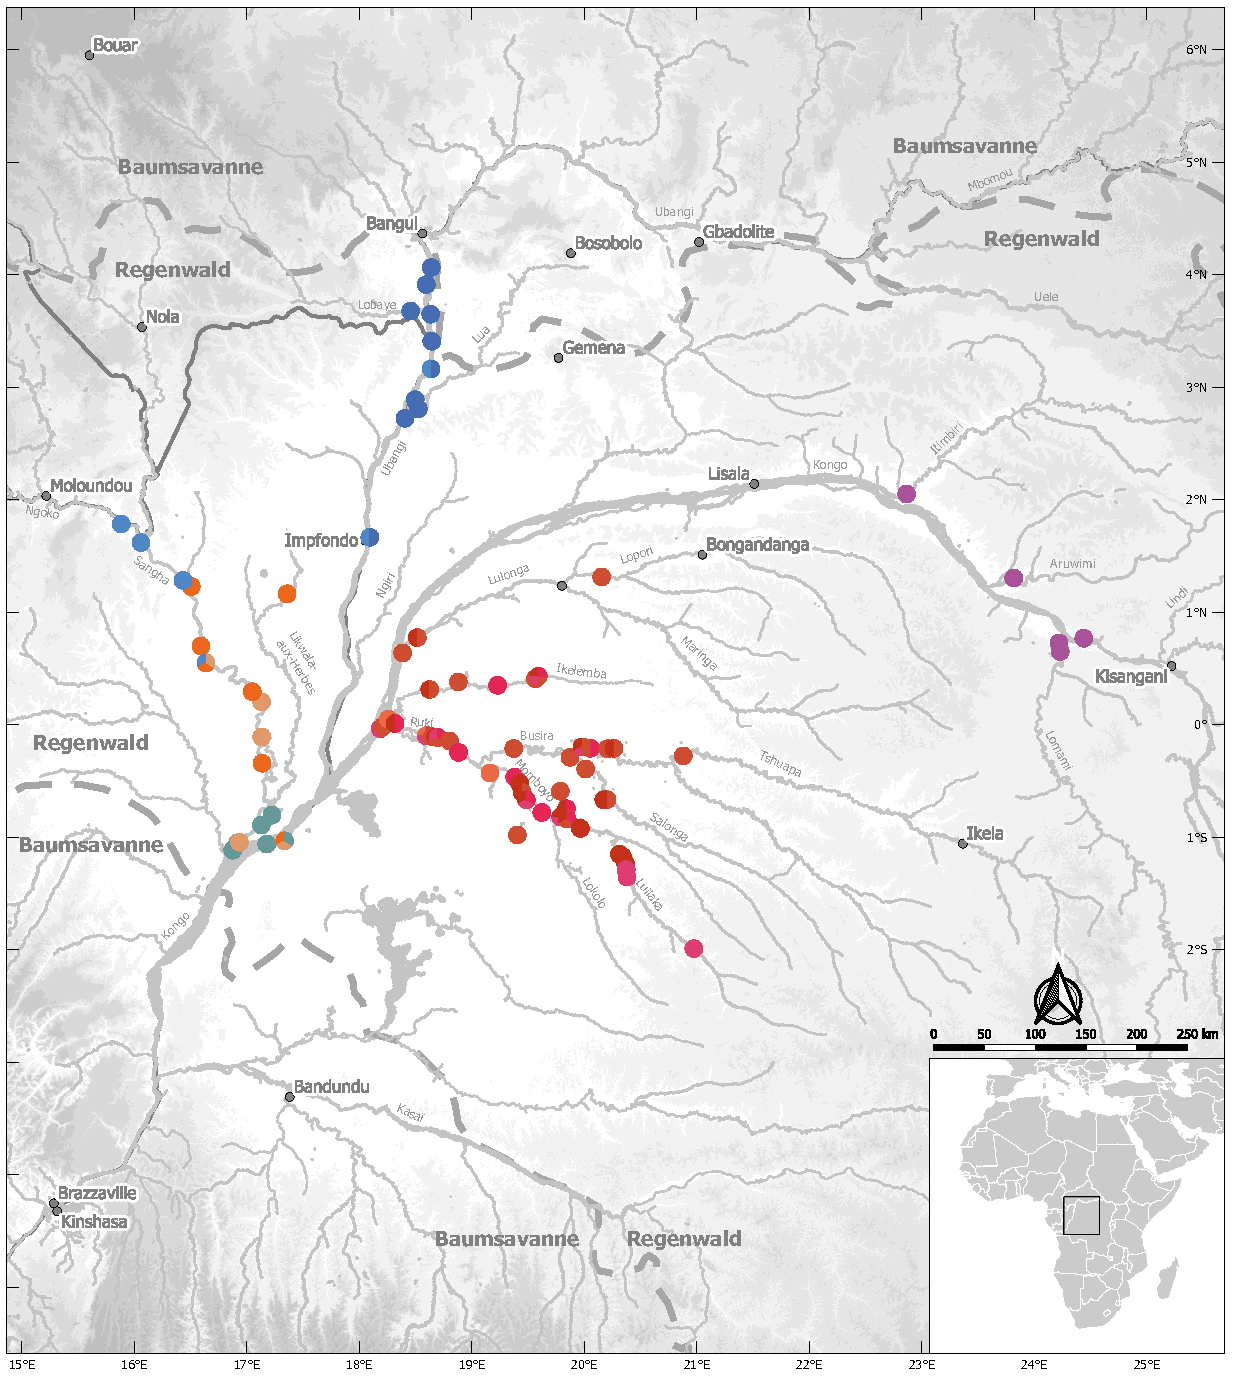
\includegraphics[width = \textwidth]{GIS/output/5-7_Zeitscheibe_EIA3_A4print-2.pdf}
		\vspace{2cm}
		\caption{Verbreitung}
		\label{fig:EIA3_Karte}
	\end{subfigure}
	\caption{Jüngere Phase der Frühe Eisenzeit (2.--6. Jh. n. Chr.).}
	\label{}
\end{figure*}
\addtocounter{figure}{-1}
\begin{figure*}[p]
	\begin{subfigure}[b]{\textwidth}
		\setcounter{subfigure}{1}
		\centering
		\includegraphics[width = \textwidth]{figs/Chronologiesystem_v3a_Zeitschiebe_EIA3.pdf}
		\caption{Chronologie}
		\label{fig:EIA3_Chronologie}
	\end{subfigure}
	\caption{Jüngere Phase der Frühe Eisenzeit (2.--6. Jh. n. Chr.).}
	\label{fig:EIA3}
\end{figure*}

Im nordwestlichen Kongobecken haben die noch bis in das 5.--6.~Jh.~n.~Chr. anzusetzenden, frühesten Stilgruppen Batalimo-Maluba (Kap.~\ref{sec:BTM-Gr}) und Pikunda-Munda (Kap.~\ref{sec:PKM-Gr}) weiterhin Bestand. Beide Gruppen spiegeln die zweigeteilte Besiedlung des Raumes wider: mit der in technischer Hinsicht stark an die Keramik des Inneren Kongobeckens angelehnten Pikunda-Munda-Keramik sowie der formal an die Oveng-Keramik aus Gabun erinnernden, technisch jedoch der Pikunda-Munda-Keramik und damit der Keramik aus dem Inneren Kongobecken entsprechenden Bokonongo-Gruppe (Kap.~\ref{sec:BOG-Gr}) im Süden (Abb.~\ref{fig:EIA3_Karte}). Im Norden findet sich weiterhin die Keramik der Batalimo-Maluba-Gruppe sowie jene der Ngbanja-Gruppe (Kap.~\ref{sec:NGB-Gr}). Das Aufkommen der Schamott-Magerung aufweisenden und formal an die Keramik von der Île des Mimosas erinnernden Bobusa-Gruppe (Kap.~\ref{sec:BBS-Gr}) kann, basierend auf dem Vergleich zu den genannten Funden aus dem Großraum Kinshasa, unter Vorbehalt in das 3.--4.~Jh.~n.~Chr. datiert werden. Die Keramik der Bobusa-Gruppe stellt ein von allen bekannten keramischen Phänomen des Kongobeckens unabhängiges Element der Besiedlungsgeschichte des Raumes dar. Gegenwärtig ist das formale Spektrum der Bobusa-Keramik zu schwach belegt und die generelle Verzierungsarmut der Stücke reduzieren den Korpus diagnostischer Merkmale weiter. Systematisch lässt sich lediglich die intentionelle Magerung mit zerstoßener Keramik anführen, die in keinem anderen Kontext im Kongobecken beobachtete werden kann. Naturräumlich kann angeführt werden, dass sich die Fundstellen der Bobusa-Gruppe nur wenige Kilometer den Kongo stromauf der heutigen südlichen Grenze des Regenwaldes befinden. Inwiefern den Kongofluss weiter stromab Funde der Bobusa-Gruppe zu erwarten sind und wo die südliche Grenze des sich potentiell noch von der Regenwaldkrise des 1.~Jt.~v.~Chr. erholenden äquatorialen Regenwalds (Kap.~\ref{sec:Palaeoumwelt}) befand, muss Gegenstand zukünftiger Forschungen bleiben und kann mit den vorliegenden Quellen nicht erörtert werden.

Im nordöstlichen Kongobecken finden sich lediglich Vertreter der Keramik der mittleren Phase (Abb.~\ref{fig:LivingstoneSmith2017_noCongoTrad}.4--7; Kap.~\ref{sec:NordCongo}). Diese ist in einem Bereich von etwa 250\,km Länge zwischen den Mündungen der Flüsse Itimbiri und Lomami verbreitet. Sie zeigt keine formalen Ähnlichkeiten zu den zeitgleichen keramischen Stilen des Inneren sowie nordwestlichen Kongobeckens und muss gegenwärtig ebenfalls als eigenständige Entwicklung angesehen werden.

\subsubsection*{Mittlere Eisenzeit (7.--10. Jh. n. Chr.)}\label{sec:MIA}

Für den Zeitraum zwischen dem 6./7. bis 11./12. Jh.~n.~Chr. liegen für weitere Teile des Kongobeckens nur sehr wenige Anzeichen einer Besiedlung in Form von Keramikfunden vor. Die Projektion der Angaben zur Chronologie der jeweiligen Stilgruppen aus dem von \textcite{Wotzka.1995} untersuchten Inneren Kongobecken auf eine absolute Zeitskala erbrachte eine auffällige Zweiteilung der dortigen Sequenz (Kap.~\ref{sec:ICB_StilGrDatierungen}). Das Ende der Stilgruppen Bokuma und Lingonda fällt in das 5.--7.~Jh.~n.~Chr. und das Aufkommen der Bondongo-Keramik kann nicht vor den Beginn des 11.~Jh.~n.~Chr. datiert werden (Kap.~\ref{sec:ICB_StilGrDatierungen}). Für die Zeit zwischen dem 7.--10.~Jh.~n.~Chr. kann \textsc{Wotzka} (ebd. 121--128) lediglich der Longa-Gruppe zuweisbare Funde anbringen (Abb. \ref{fig:14C_InnerCongo_Stylegroups}.1--3). Die Funde dieses Stils zeichnen sich einerseits durch einen zwischen der älteren Keramik der Stile Bokuma sowie Bokele und den jüngeren, der Bondongo-Keramik nahestehenden Stile stilistisch überbrückenden Charakter aus. Andererseits lieferten die drei mit Longa-Keramik assoziierten Radiokohlenstoffdatierungen \textsc{Wotzka} (ebd. 127f. mit Tab.~53) aufgrund ihrer massiven Streuung nur unzureichende absolute Datierungsindizien. In einer 2015 entstandenen Zusammenstellung von Typentafeln für die Stilgruppen des Inneren Kongobeckens gibt Wotzka dem jüngsten, in das späte 12.--13.~Jh.~n.~Chr. fallenden Datum den Vorzug von den beiden anderen, deutlich älteren.\footnote{Siehe Anm.~\ref{ftn:fstafrikaWebStilGr-Tafeln}.} Eine \enquote*{Überbrückung} der im 6.--7.~Jh.~n.~Chr. abbrechenden Sequenz zum jüngeren, im 11.--12.~Jh.~n.~Chr. einsetzenden Abschnitt kann im Lichte dieser Entwicklungen nur noch schwer aufrechterhalten werden (Abb.~\ref{fig:Chronologiesystem}).\footnote{Siehe Anm.~\ref{ftn:LON-Flaschenhals}.} 

Anzeiger für Aktivitäten prähistorischer Gruppen im 7.--10.~Jh.~n.~Chr. sind auch im nordwestlichen Kongobecken äußerst selten. Die Nachweise für die älteren Stile Batalimo-Maluba (Kap. \ref{sec:BTM-Gr}), Ngbanja (Kap.~\ref{sec:NGB-Gr}), Pikunda-Munda (Kap.~\ref{sec:PKM-Gr}) und Bokonongo (Kap. \ref{sec:BOG-Gr}) brechen sämtlich im 5.--6.~Jh.~Chr. ab. Entlang des mittleren Ubangi können lediglich Vertreter der nicht absolut datierbaren Stilgruppen Dongo (Kap.~\ref{sec:DON-Gr}) und Mokelo (Kap.~\ref{sec:MKL-Gr}) potentiell dieser Phase zugerechnet werden. Diese Ansprache gründet jedoch gänzlich in dem stilistisch überbrückenden Charakter der beiden Stile, die die ältere Keramik der Stile Batalimo-Maluba (Kap.~\ref{sec:BTM-Gr}) und Ngbanja (Kap.~\ref{sec:NGB-Gr}) mit der jüngeren Motenge-Boma-Keramik (Kap.~\ref{sec:MTB-Gr}) verbindet. Da es sich hierbei jedoch um einzelne Ähnlichkeiten auf Merkmalsebene handelt, müssen diese Angaben mit höchster Vorsicht betrachtet werden und eine sichere chronologische Ansprache der beiden Stile kann nur durch zusätzliche Geländearbeit erfolgen.

\begin{figure*}[p]
	\centering
	\begin{subfigure}[b]{\textwidth}
		\centering
		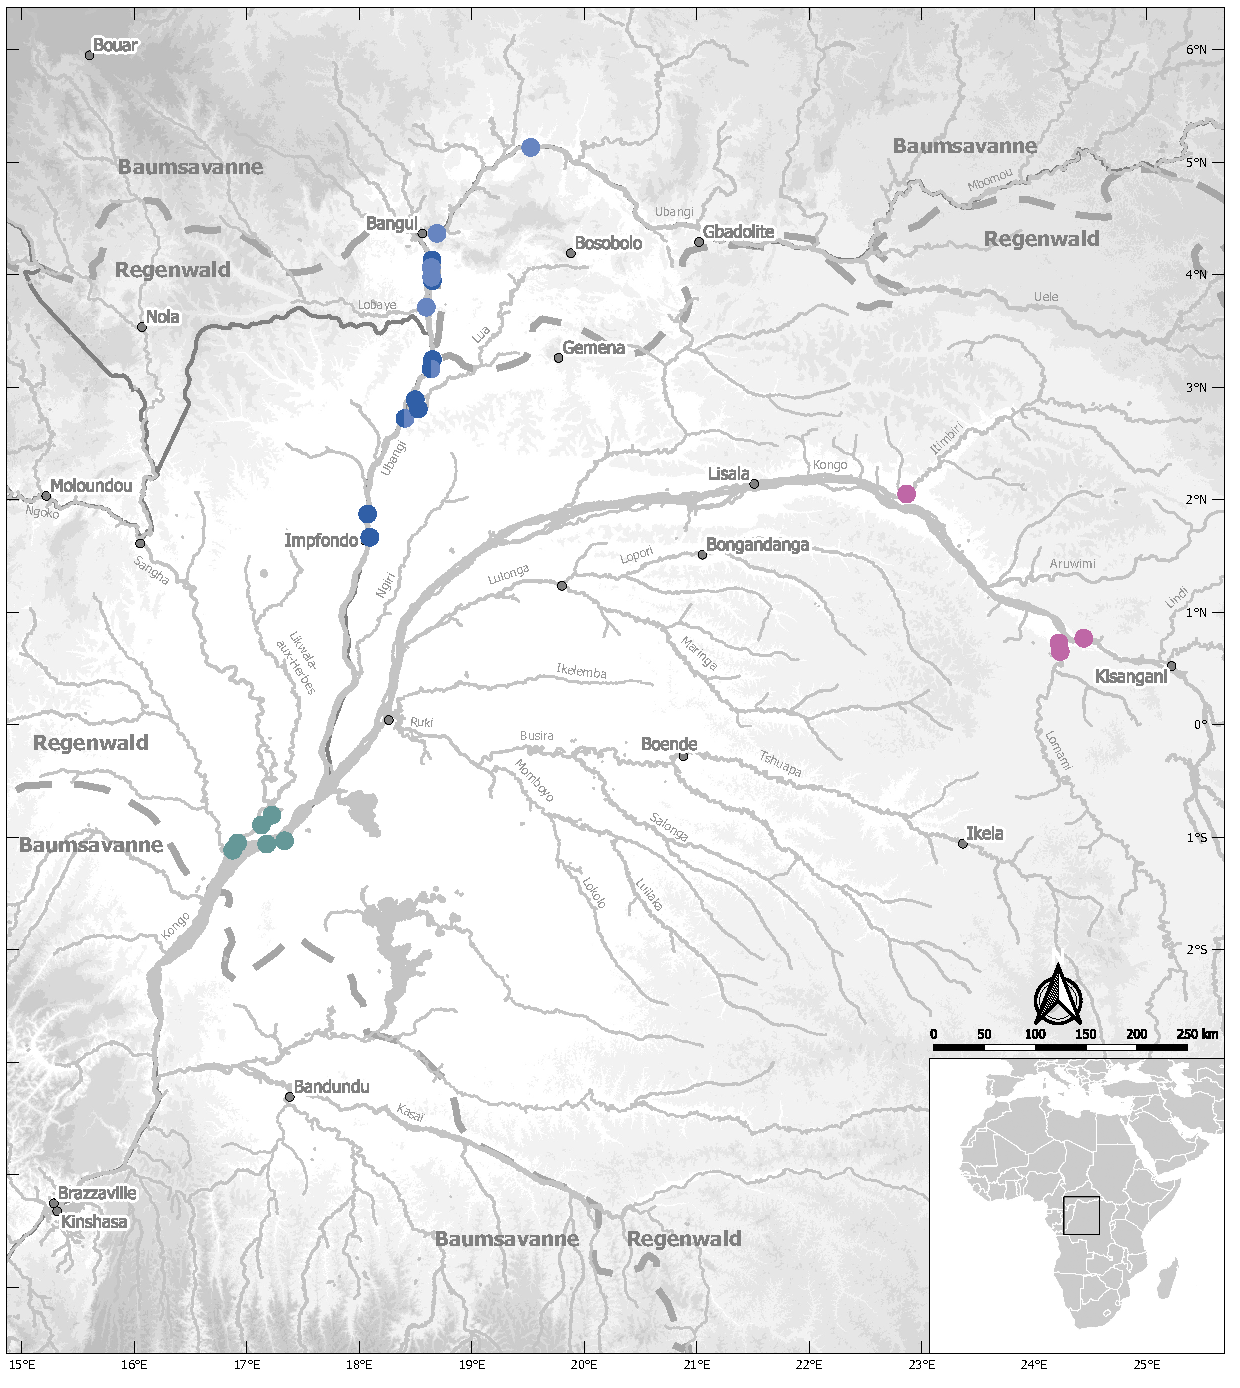
\includegraphics[width = \textwidth]{GIS/output/5-7_Zeitscheibe_MIA_A4print-2.pdf}
		\vspace{2cm}
		\caption{Verbreitung}
		\label{fig:MIA_Karte}
	\end{subfigure}
	\caption{Mittlere Eisenzeit (7.--10. Jh. n. Chr.).}
	\label{}
\end{figure*}
\addtocounter{figure}{-1}
\begin{figure*}[p]
	\begin{subfigure}[b]{\textwidth}
		\setcounter{subfigure}{1}
		\centering
		\includegraphics[width = \textwidth]{figs/Chronologiesystem_v3a_Zeitschiebe_MIA.pdf}
		\caption{Chronologie}
		\label{fig:MIA_Chronologie}
	\end{subfigure}
	\caption{Mittlere Eisenzeit (7.--10. Jh. n. Chr.).}
	\label{fig:MIA}
\end{figure*}

Keramik der am mittleren Ubangi und Sangha sowie Likwala-aux-Herbes verbreitet Matoto-Gruppe fand sich lediglich in einem datierbaren Befund; im Zusammenhang mit der Sekundärbestattung MLB~85/1-4-3 (Kat.-Nr.~3). Dieser Befund kann auf Basis von zwei Radiokohlenstoffdatierungen in das 11.--15.~Jh.~n.~Chr. datiert werden. Die Matoto-Keramik muss potentiell mit der Verfüllung der Eingrabung in Zusammenhang gebracht werden und müsste folglich mindestens zeitgleich oder älter als der Befund sein. Entsprechend kann die Keramik der Matoto-Gruppe sowohl in die Mittlere Eisenzeit als auch die ältere Phase der späten Eisenzeit datieren.

Am südlichen Rand des nordwestlichen Kongobeckens, dem Mündungsbereich des Sangha, kann noch von einem bis in das 7.~Jh.~n.~Chr. hineinreichenden Weiterbestehen der Bobusa-Keramik ausgegangen werden (Kap.~\ref{sec:BBS-Gr}). Jedoch stützt sich auch diese Ansprache lediglich auf starke technische sowie schwache formale Ähnlichkeiten zur Keramik der am Pool Malebo gelegenen Île des Mimosas (Abb.~\ref{fig:Niederkongo_Sequence}.7--9). Die Funde von der Île des Mimosas sind Teil der von \textcites{deMaret.1986}{Maret.1990} beschriebenen Gombe-Gruppe, die auf Basis von vier Radiokohlenstoffdatierungen in das 3.--7.~Jh.~n.~Chr. datiert werden kann (Abb.~\ref{fig:14C_Niederkongo}).

Im nordöstlichen Kongobecken enden im 4.~Jh.~n.~Chr. auch die Belege für Keramik der mittleren Phase (Kap.~\ref{sec:NordCongo}). Jedoch lassen sich Funde der Ilambi-Gruppe mit einem in das 8.--10.~Jh.~n.~Chr. datierenden Radiokohlenstoffdatum in Zusammenhang bringen \parencite[4 Tab.~1: Poz-75462]{LivingstoneSmith.2017}. Die Ilambi-Keramik zeigt ein ähnliches Verbreitungsbild wie die Keramik der ihr vorangegangen mittleren Phase. Jedoch markiert das Aufkommen der Ilambi-Keramik im 8.--10.~Jh.~n.~Chr. einen auffälligen Bruch in der keramischen Entwicklung der Region. Die Keramik der älteren und mittleren Phase, die in Aufbauttechnik produziert wurden und ein Dekor aus Riefen, Rillen und Eindrücken aufweisen, werden von in Abformtechnik hergestellten und rouletteverzierten Gefäßen abgelöst. Es kann beim gegenwärtigen Stand der Untersuchungen nur der Zusammenfall des beschriebenen mutmaßlichen Abbruchs der Siedlungsaktivität in weiten Teilen des Kongobeckens mit dem von \textcite{LivingstoneSmith.2017} beobachteten Technologiewechsel konstatiert werden. Diachrone Betrachtungen zur Keramiktechnologie liegen lediglich für das nordöstliche Kongobecken (Kap.~\ref{sec:NordCongo}) vor, während für das nordwestliche Kongobecken lediglich ein erster, nur bedingt systematischer Einblick in die Entwicklungsgeschichte der Töpfereitechnik existiert (Kap.~\ref{sec:Herstellung}). Jedoch unterstreichen die dahingehenden Ergebnisse von \textcite{LivingstoneSmith.2017} aus dem nordöstlichen Kongobecken das Potential entsprechender Untersuchungen.

Ein breites mit einem Rückgang oder gar Abbruch der Siedlungsaktivitäten verbundenen Phänomens innerhalb der mittleren Eisenzeit in Zentralafrika wurde mehrfach von \textcites[101--103~Abb.~9]{Oslisly.1998}[112f.~Abb.~7.9]{Oslisly.2001d}{Oslisly.2013}{Oslisly.2013b} diskutiert. Belege für in der zweiten Hälfte des 1.~Jt.~n.~Chr. zu beobachtende Abbrüche lokaler oder regionaler Sequenzen sind auch aus anderen Teilen Zentralafrikas bekannt. So berichtet \textcite{Leka.2008} von einer zwischen das 1.--13.~Jh.~n.~Chr. reichenden Lücke in der aus elf Radiokohlenstoffdatierungen bestehenden Sequenz für eine Reihe nördlich der kamerunischen Hauptstadt Yaoundé gelegener Fundstellen. Auch an der südöstlich von Douala, im Westen Kameruns gelegenen Fundstelle Dibamba ließen sich zwischen den im 4.~Jh.~n.~Chr. endenden Befunden der frühen Eisenzeit und den ab dem 10.~Jh.~n.~Chr. belegten späteisenzeitlichen Strukturen keine Befunde nachweisen \parencites{Oslisly.2008}[377--380, 379 Abb.~36.6]{GouemGouem.20102011}. Auch die Sequenz der vor Äquatorialguinea gelegenen kleinen Insel Corsico weist eine auffällige Lücke auf (Kap.~\ref{sec:Gabun}). \textcite[355f.]{SanchezElipe.2016} weisen explizit darauf hin, dass aus dem Zeitraum zwischen dem Ende der späten Oveng-Keramik im 8.~Jh.~n.~Chr. und dem Aufkommen der Nandá-Keramik ab dem 10./11.~Jh.~n.~Chr. weder Gräber noch Siedlungsbefunde bekannt sind. Sie gehen für diese drei Jahrhunderten sogar davon aus, dass die Insel unbewohnt war. Zwischen dem 7.--10.~Jh.~n.~Chr. lässt sich folglich nicht nur im hier systematisch betrachteten Kongobecken ein Rückgang bis potentiell sogar Abbruch der Anzeiger für Siedlungsaktivitäten beobachten.\footnote{Der Rückgang archäologischer Zeugnisse im vorliegenden Korpus an Funden und Befunden im Kongobecken fällt zeitlich grob mit der gegenwärtig nur bedingt nachvollzogenen \textit{Late Antique Little Ice Age} beziehungsweise dem \enquote*{A.D. 536}-Klimaevent zusammen \parencites[siehe][]{Larsen.2008}{Buntgen.2016}. \textcite[337]{Hubau.2013} beschreiben für den Zeitraum im Anschluss an das Ende der \enquote*{Regenwaldkrise} des 1.~Jt.~v.~Chr. (siehe Kap.~\ref{sec:Palaeoumwelt}) eine Regenerationsphase des Regenwaldes im Zuge eines zunehmend feuchteren, stabilen Klimas. In Ostafrika sowie an der Atlantikküste  lassen sich Veränderungen gegenwärtig erst wieder mit dem Beginn der Kleinen Eiszeit in der ersten Hälfte des 14.~Jh.~n.~Chr. fassen.}

\subsubsection*{Ältere Phase der Späten Eisenzeit (11.--16. Jh. n. Chr.)}

Im Anschluss an die geschilderte potentielle Abnahme oder sogar Unterbrechung der Siedlungsaktivität während der Mittleren Eisenzeit können ab dem 11.~Jh.~n.~Chr. wieder eindeutige Zeugnisse einer breiten Aufsiedlung des Kongobeckens beobachtet werden. Im Inneren Kongobecken wird diese vor allem durch die nahezu im gesamten von \textcite{Wotzka.1995} bearbeiteten Raum verbreiteten Stilgruppen Longa (ebd. 558f. Karte~9; Abb.~\ref{fig:Wotzka1995_TypenICB_LIA1}.1--3) und Bondongo (ebd. 562f. Karte~11; Abb.~\ref{fig:Wotzka1995_TypenICB_LIA1}.4--9) getragen. Beide Stile zeichnen sich durch eine elaborierte Verzierung aus, im Fall der Bondongo-Keramik umfasst diese eine besondere Hervorhebung der häufig plastisch ausgearbeiteten Schulterpartie der Gefäße. Die Keramik zeichnet sich -- soweit die diesbezüglich untersuchten Stichproben herangezogen werden können\footnote{Siehe Kap.~\ref{sec:Herstellung2_Fabric}.} -- vor allem durch die \textit{Fabrics} 1 und 2 aus. Anstatt vor allem flacher Böden werden innerhalb der Stilgruppen der Späten Eisenzeit jedoch vornehmlich runde Böden hergestellt (Tab.~\ref{fig:Wotzka1995Bodenformen}).\footnote{Während die Keramik der in die jüngere Phase der Frühen Eisenzeit datierenden Stilgruppen Bokuma und Lingonda noch Anteile runder Böden von unter 8\,\% aufwiesen, liegt er innerhalb der Stilgruppen Longa und Bondongo bei zwischen 67--70\,\% (Tab.~\ref{fig:Wotzka1995Bodenformen}). Ein entsprechender stringenter Wandel von flachen zu runden Böden lässt sich im nordwestlichen Kongobecken nicht beobachten. Mit Blick auf die Besiedlungsgeschichte des Inneren Kongobeckens muss jedoch der Tatsache, dass die Stilgruppen der Älteren Eisenzeit durchweg flache Boden zeigen, während sich die Stile der Späteren Eisenzeit zu großen Teilen durch runde Böden auszeichnen, wie sie auch für die rezenten Töpfereibelege nachgewiesen sind \parencite{Eggert.1980c}, eine nicht zu vernachlässigende Bedeutung zugesprochen werden.} Innerhalb der beginnenden Späten Eisenzeit lässt sich innerhalb der keramischen Entwicklung des Inneren Kongobeckens zudem eine Verzweigung der von \textcite[221--223]{Wotzka.1995} beschriebenen \textit{West-Tradition} in eigenständige, lokal geprägte Stiltraditionen am Luilaka sowie Tshuapa beobachten. Die im Süden des Inneren Kongobeckens verbreitete \textit{Luilaka-Tradition} wird aus den Stilgruppen Bekongo und Wafanya gebildet. \textcite{Wotzka.1995} attestiert ihr einen eigenständigen aber kurzlebigen Charakter. Der Bekongo-Stil spiegelt eine lokale Entwicklung der Longa-Keramik wider, die aber auch deutliche Bezüge zur Bondongo-Keramik aufweist und aus dem sich der Wanfanya-Stil entwickelt. Gegen Ende der Bondongo-Keramik im 13.--15.~Jh.~n.~Chr. wird von Wotzka (ebd. 222f.) auch im Gebiet des Tshuapa, im Osten des Inneren Kongobeckens \textsc{eine} einsetzende Regionalisierung konstatiert. Diese Entwicklung setzt mit dem Wema-Stil im 13.--14.~Jh.~n.~Chr. ein und lässt sich bis zur rezenten Ilemba-Bokonda-Keramik nachvollziehen (Kap.~\ref{sec:ICB_StilGrDatierungen}). Die bislang ältesten publizierten Belege für die Nutzung von Eisen im Inneren Kongobecken stammen aus mit Keramik der Bondongo-Gruppe assozzierten Fundzusammenhängen (ebd. 288).\footnote{Siehe auch Anm.~\ref{ftn:EisenIYO15/2-4}} 

\begin{figure*}[p]
	\centering
	\begin{subfigure}[b]{\textwidth}
		\centering
		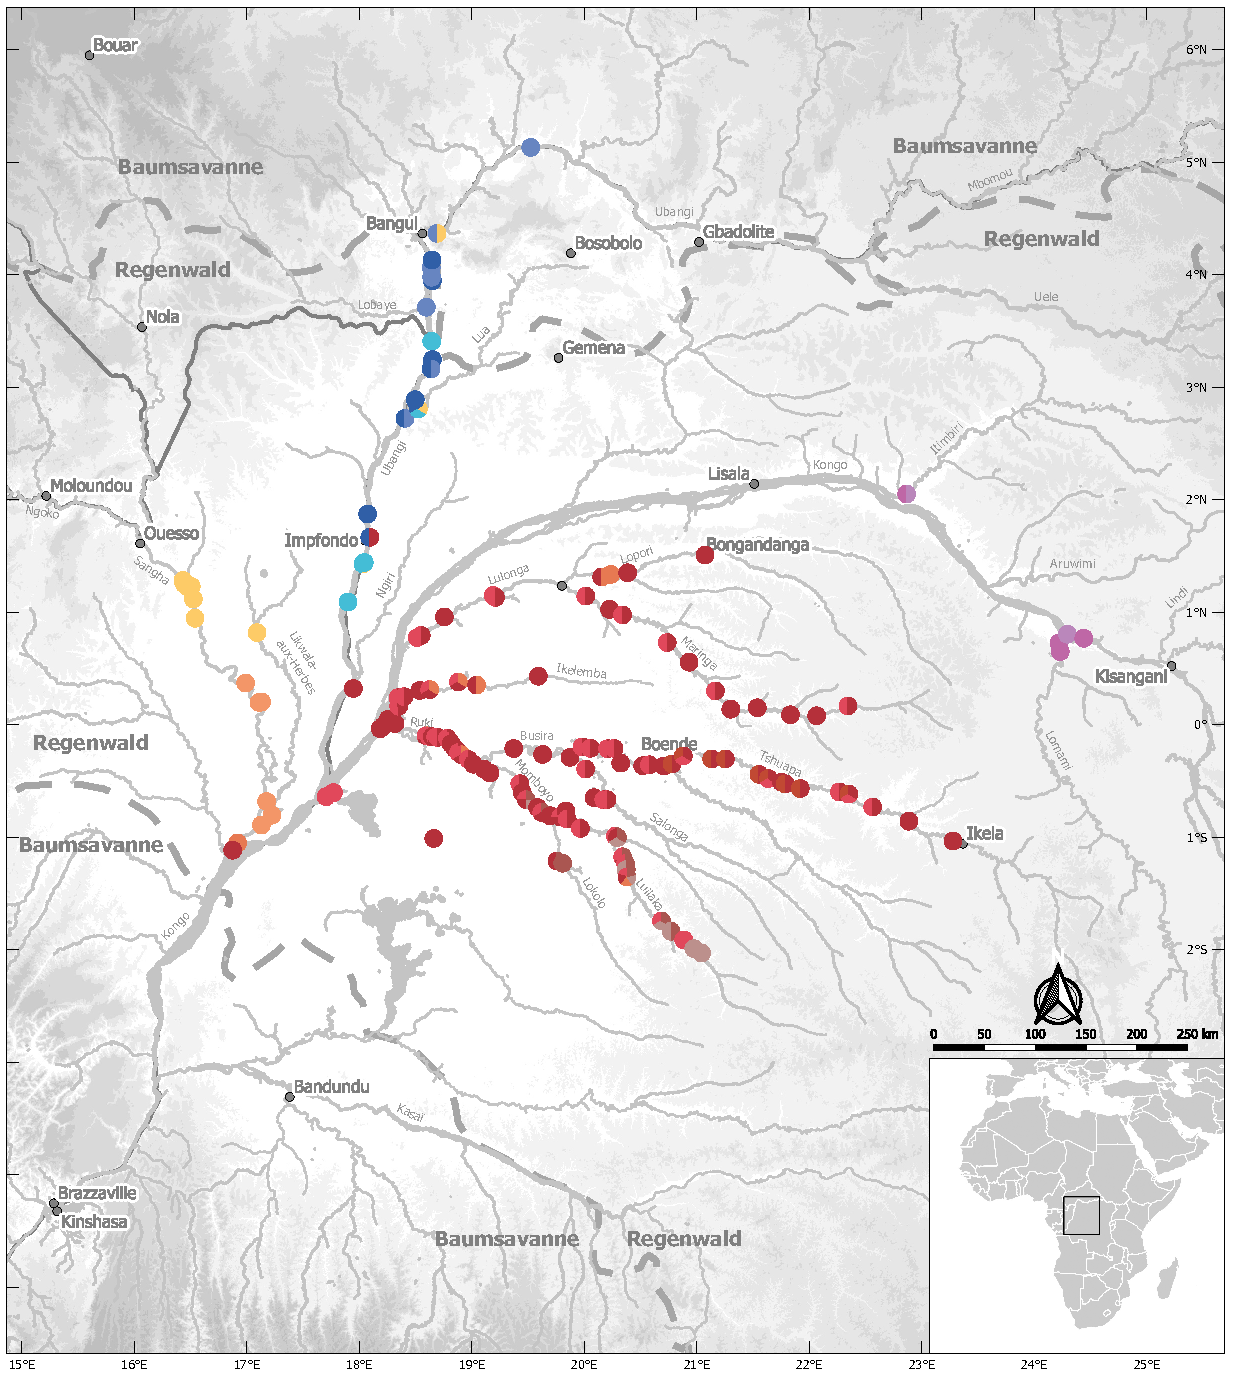
\includegraphics[width = \textwidth]{GIS/output/5-7_Zeitscheibe_LIA1_A4print-2.pdf}
		\vspace{2cm}
		\caption{Verbreitung}
		\label{fig:LIA1_Karte}
	\end{subfigure}
	\caption{Ältere Phase der Späten Eisenzeit (10.--16. Jh. n. Chr.).}
	\label{}
\end{figure*}
\addtocounter{figure}{-1}
\begin{figure*}[p]
	\begin{subfigure}[b]{\textwidth}
		\setcounter{subfigure}{1}
		\centering
		\includegraphics[width = \textwidth]{figs/Chronologiesystem_v3a_Zeitschiebe_LIA1.pdf}
		\caption{Chronologie}
		\label{fig:LIA1_Chronologie}
	\end{subfigure}
	\caption{Ältere Phase der Späten Eisenzeit (10.--16. Jh. n. Chr.).}
	\label{fig:LIA1}
\end{figure*}

Im südlichen Teil des nordwestlichen Kongobeckens findet sich die Ngombe-Gruppe, die -- trotz fehlender Radiokohlenstoffdatierungen -- aufgrund ihrer starken Ähnlichkeiten zu den aus dem Inneren Kongobecken bekannten Stilen Longa und Mbandaka grob in das 12.--13.~Jh.~n.~Chr. datiert werden kann (Kap.~\ref{sec:NGO-Gr}). Die Ngombe-Keramik spiegelt eindeutig eine lokale Entwicklung der \textit{West-Tradition} des Inneren Kongobeckens wider und deutet begrenzte Siedlungsaktivitäten entlang des unteren Sangha an. Ähnlich ist auch die entlang des unteren Ubangi verbreitete Bokwango-Keramik zu bewerten, die ebenfalls starke formale Bezüge zur Keramik der Stilgruppen Mbandaka und Nkile aus dem Inneren Kongobecken aufweist (Kap.~\ref{sec:BKW-Gr}). Weiter nördlich, den Ubangi stromauf finden sich weiterhin die potentiell bereits seit der Mittleren Eisenzeit bekannten Stile Dongo (Kap.~\ref{sec:DON-Gr}) und Mokelo (Kap.~\ref{sec:MKL-Gr}), zu denen ab der Späten Eisenzeit noch die Stilgruppe Bobulu (Kap.~\ref{sec:BBL-Gr}) hinzugerechnet werden kann. Grob an den Übergang des älteren zum mittleren Abschnitts der Späten Eisenzeit im 16.--17.~Jh.~n.~Chr. lässt sich die Keramik der Motenge-Boma-Gruppe stellen, die ein auffällig stark abgegrenztes Verbreitungsgebiet zwischen der Lua-Mündung und dem Ubangi-Bogen aufweist (Kap.~\ref{sec:MTB-Gr}). Bereits mit den Stilen Dongo und Mokelo sind vereinzelte Hinweise auf die Nutzung von Rouletteverzierung bekannt, die ab der Motenge-Boma-Keramik zur bestimmenden Verzierungstechnik der Keramik am mittleren und oberen Ubangi wird. Im westlichen Teil des nordwestlichen Kongobeckens, entlang des oberen Sangha und Ngoko lässt sich ab dem 13.--14.~Jh.~n.~Chr. erstmals eine massive Siedlungsaktivität in Form der aufkommenden \textit{Ngoko-Tradition} nachweisen. Die älteste und einzige direkt datierte Ausprägung dieser Stilgruppe stellt die Mandombe-Keramik dar (Kap.~\ref{sec:MDB-Gr}), deren Fokus auf stark bauchige Gefäße mit kurzen Zylinderhälsen und einem auf Kammstrich und Appliquen basierenden Dekor keine Vorläufer im keramischen Fundgut des nordwestlichen Kongobeckens hat. Aus der mutmaßlich zeitgleichen bis leicht jüngeren Keramik der Konda-Gruppe sind erst Belege für die Nutzung von Rouletteverzierung bekannt (Kap.~\ref{sec:KON-Gr}). Wie auch entlang des Ubangi lässt sich innerhalb der älteren Phase der Späten Eisenzeit auch am Sangha und Ngoko eine gelegentliche und nicht das Verzierungsspektrum der entsprechenden Stile bestimmende Nutzung von Rouletteverzierung beobachten. Erst am Übergang zur mittleren Phase der Späten Eisenzeit finden sich Stilgruppen wie die Motengo-Boma-Gruppe am Ubangi (Kap.~\ref{sec:MTB-Gr}) sowie die Pandama-Gruppe am oberen Sangh und Ngoko (Kap.~\ref{sec:PDM-Gr}), in denen Rouletteverzierung die bestimmende Verzierungstechnik bildet.

Die frühesten Nachweise für die Roulettetechnik stammen aus Westafrika und datieren in das 2.~Jt.~v.~Chr. \parencite[189]{LivingstoneSmith.2007}. Im Laufe der folgenden Jahrhunderte ist eine Ausbreitung von Rouletteverzierungen über den gesamten nördlichen Sahel, vom Senegal im Westen bis in die Region der großen Seen in Ostafrika zu beobachten (ebd. 203 Abb.~9). Verschiedene frühere Studien haben in der Ausbreitung der Rouletteverzierung tiefgreifende Veränderungen für die jeweiligen Regionen gesehen und diese häufig mit der Verbreitung bestimmter linguistischer Gruppen in Zusammenhang gebracht. So wurde zum Beispiel die Ausbreitung von Schnitzroulette als materieller Marker der Adamawa-Ubangi-Sprachen gewertet \parencite{David.1977}. In ihrer Analyse von linguistischen Veränderungen und Rouletteverzierung in der Uele-Region der Demokratischen Republik Kongo sowie den Bezeichnungen für Gegenstände, die bei der Keramikherstellung genutzt werden und Rouletteverzierungen in der Karanga-Region Tansanias spricht sich Mary \textcite{McMaster.2005} gegen die Möglichkeit aus, dass Diffusion der treibende Faktor der Ausbreitung der Rouletteverzierung sei. Bei Betrachtung der zur Verfügung stehenden Radiokohlenstoffdatierungen für die Einführung der Rou\-lette\-ver\-zier\-ung in die Region der großen Seen scheint aber auch eine simple Einführung durch Migration wenig wahrscheinlich (ebd. 63). Nichts desto trotz sieht \textcite{McMaster.2005} in der Einführung der Rouletteverzierung einen Wendepunkt in der regionalen Besiedlungsgeschichte. Zu anderen Schlüssen kommt Ceri \textcite{Ashley.2010}, die eine keramische Übergangsphase zwischen der Urewe-Keramik, der ältesten keramischer Stilgruppe des Gebiets zwischen den großen Seen, und der jüngeren mit vegetabilischem Roulette verzierten Ware aufzeigen kann. Der Übergang, wie er von \textcite{Ashley.2010} beschrieben wird, vollzieht sich im 10.~Jh.~n.~Chr., wenn weniger aufwendige Formen mit klaren Bezügen zur älteren Urewe-Keramik, durch nicht-rouletteverzierte Formen abgelöst werden \parencite[890f.]{Reid.2013}. Diese werden in der ersten Hälfte des 2.~Jt.~n.~Chr. durch ähnliche Formen, die nun aber \textit{twisted string}-Roulette und breite Rillen zeigen und als Entebbe-Gruppe bezeichnet werden, abgelöst. Die Entebbe-Keramik leitet in der Folge zu den typischen, rouletteverzierten Formen der Region über. Für \textcite{Ashley.2010} ergibt sich durch die Einführung der Rouletteverzierung kein Bruch in der Sequenz. Im nordwestlichen Kongobecken bildet Rouletteverzierung ebenfalls ein leicht ansprechbares Charakteristikum, das jedoch als Anzeiger für einen tiefgreifenden Wandel fehlinterpretiert werden kann.

Nachvollziehbar wird der Prozesse, der mit der Einführung der Roulettekeramik in das nordwestliche Kongobecken einhergeht unter anderem anhand des Grabungsbefundes PIK~87/1 in Pikunda am Sangha (Kat.-Nr. 8). Die jüngere Grube A, die bis etwa 1\,m unter die Oberfläche reicht, enthielt vornehmlich Keramik der Mandombe-Gruppe (Kap.~\ref{sec:MDB-Gr}). Diese Keramik steht formal in einem starken Kontrast zu der in der zweiten, älteren im Schnitt PIK~87/1 nachgewiesenen Grube, die Pikunda-Munda-Keramik enthielt (Kap.~\ref{sec:PKM-Gr}). Beide Gruben sind mit jeweils einer Radiokohlenstoffprobe datiert und während die Pikunda-Munda-Keramik in das 4.~Jh.~v.~Chr.--3./4.~Jh.~n.~Chr. datiert, stammt die Mandombe-Keramik aus dem 12.--14.~Jh.~n.~Chr. Während sich die Mandombe-Keramik mit Blick auf Formen, Verzierungen und \textit{Fabrics} von der vor ihr in Pikunda nachgewiesenen Keramik der Pikunda-Munda-Gruppe unterscheidet, zeigt sie große Ähnlichkeiten zu den Stilgruppen Konda (Kap.~\ref{sec:KON-Gr}) und Pandama (Kap.~\ref{sec:PDM-Gr}). Die Ähnlichkeiten im Bezug auf die formalen Charakteristika, wie die stark bauchige Gefäße mit kurzem Hals, und Hinweise auf eine ähnliche Technologie (Kap.~\ref{sec:Herstellung}) schließt jedoch nicht die Dokrationspraxis mit ein. Die Mandombe-Keramik zeigt vor allem diagonalen Kammstrich sowie Kammeindrücke und plastische Element auf den Gefäßoberteilen und häufig ein schlickergerautes Gefäßunterteil. Die Konda-Keramik hingegen weist keine plastischen Elemente oder Schlickerrauung auf. Ihre Verzierungen bestehen fast ausschließlich aus Rillen. Markant sind vor allem die innen wie außen gerillten Ränder. Sechs der Konda-Gruppe zurechenbare Stücke zeigen jedoch überdies und neben dem charakteristischen Rillendekor auch Rouletteverzierung. Die Pandama-Keramik nun zeichnet sich regelhaft durch eine Kombination von flächigem \textit{knotted strip}-Roulette aus, welches von überkreuzten Rillen überlagert wird. Für die beiden letztgenannten Gruppen liegen keine absoluten Datierungen vor, doch weisen sie stilistisch den Weg von der Mandombe-Keramik des 12.--14.~Jh.~n.~Chr. zur rezenten Mbenja-Keramik (Kap.~\ref{sec:MBJ-Gr}) und werden daher als chronologisch zwischen diesen beiden Gruppen stehend angesehen. Das Aufkommen der \textit{Ngoko-Tradition} ist jedoch nicht mit dem Aufkommen der Rouletteverzierung gleichzusetzen. Diese tritt erst zur Zeit der Pandama-Gruppe deutlich hervor. Es kann daher festgehalten werden, das im westlichen Teil des Arbeitsgebietes, im Bereich des oberen Sangha und Ngoko die Rouletteverzierung in ein bestehendes keramisches System aufgenommen wurde. Grundsätzliche Änderungen, mit Blick auf keramische Grundformen, \textit{Fabrics} oder grundsätzlicher Verzierungsstruktur, lassen sich zwischen der Keramik der Mandombe-, Konda und Pandama-Gruppe nur selten beobachten. Folglich bildet die Einführung von Roulette in diesem Gebiet auch keinen Wendepunkt in der keramischen Sequenz und lässt sich somit nicht im Sinne von Änderungen der ansässigen Bevölkerungen oder linguistischer Gruppen interpretieren. Eine ganz ähnliche Situation deutet sich auch entlang des Ubangi an, wo sich innerhalb der Stile Dongo (Kap.~\ref{sec:DON-Gr}) und Mokelo (Kap.~\ref{sec:MKL-Gr}) eine auf Einzelfälle beschränkte und in die bestehenden Verzierungsgewohnheiten der beiden Stile integrierte Nutzung von Roulette beobachten lässt, während eine breite und dominierende Verwendung erst in einem späteren Schritt, innerhalb der Motengo-Boma-Gruppe beobachtet werden kann.
% \parencite[1381]{Oslisly.2013b}: LIA startet im 11. Jh. n. Chr.

Im nordöstlichen Kongobecken ist die diskutierte Einführung von Roulette ebenfalls mit der älteren Phase der Späten Eisenzeit zu assoziieren (Kap.~\ref{sec:NordCongo}). Innerhalb der auf Basis zweier Radiokohlenstoffdatierungen zwischen das 8.--10.~Jh.~n.~Chr. sowie 15.--17. Jh.~n.~Chr. datierenden Ilambi-Keramik zeigen sich erste Hinweise für potentielle Rouletteverzierung. \textcite[17, 19 Abb.~26]{LivingstoneSmith.2017} sind sich jedoch unsicher ob es sich bei den entsprechenden Verzierungselementen um ein aus mehreren hölzernen Kernen bestehendes mit Schnur umwickeltes Roulette oder Mattenabdruck handelt. Die potentiell jüngere Yaekela-Keramik zeichnet sich hingegen durch ein vornehmlich aus Schnitzroulette bestehendes Dekor aus. Die Gefäße der Ilambi-Gruppe wie jene der Yaekela-Gruppe zeigen, neben dem Wechsel der Verzierungspraxis, auch einen Wandel in der Herstellungstechnik an: eine Ablösung der in Aufbautechnik hergestellten Keramik der Älteren Eisenzeit durch in Abformtechnik getöpferte Gefäße. Mit Blick auf den aktuellen Stand der Auswertung muss jedoch offen bleiben, ob im nordöstlichen Kongobecken der beobachtete Wandel der Herstellungstechnik auch sicher mit der Einführung von Roulettedekor zusammenfällt oder ob zwischen Ilambi- und Yaekela-Keramik eher eine sukzessive Übernahme stattfand.

\subsubsection*{Mittlere Phase der Späten Eisenzeit (17.--19. Jh. n. Chr.)}

Ab dem 16.--17.~Jh.~n.~Chr. lässt sich ein weiterer Wechsel in den keramischen Inventaren beobachten. Im Inneren Kongobecken zeigt sich dieser im Ende der Stile, die nachweislich von den Stilgruppen Bondongo und Nkile geprägt sind; zwei Stilgruppen die jeweils ein Reihe an regionalen Ausprägungen hervorgebracht haben \parencite[224f.]{Wotzka.1995}.\footnote{Die Stilgruppen Bondongo, Bekongo, Wafnaya, Besongo und Wema lassen sich aufgrund jeweils charakteristischer Gefäßformen mit prononcierten Schulterpartien sowie Fisch- beziehungsweise Kauri-Motiven und Girlandenzier einem \textit{Bondongoid-Horizont} zuweisen. Dieser überschneidet sich zeitlich mit einem etwas jüngeren, sich durch charakteristische Kugeltopfformen auszeichnenden Stilen Nkile, Malelembe, Bosanga und Bolondo sowie Mpokioko gebildeten \textit{Nkiloid-Hoizont} (ebd. 224f.; Kap.~\ref{sec:Horizonte}).} Im Westen des Inneren Kongobeckens wird die heterogene keramische Entwicklung der älteren Phase der Späten Eisenzeit durch die Botendo-Keramik abgelöst (Abb.~\ref{fig:Wotzka1995_TypenICB_EIA1}.16--18), die mit ihrem bereits deutlich verarmten Verzierungsspektrum, das fast nur noch aus flächigem \textit{banfwa-nfwa} auf den Wandungen und breiten Rillen im Hals- und Randbereich besteht, direkt zur rezenten Ikenge-Keramik überleitet (Abb.~\ref{fig:Wotzka1995_TypenICB_EIA1}.19--22). Keramik der Botendo-Gruppe findet sich aber nicht nur im Inneren Kongobecken sondern auch im Süden des nordwestlichen Kongobeckens, entlang des unteren Ubangi und Likwala-aux-Herbes. Im Osten des Inneren Kongobeckens, entlang des Tshuapa hat die gleichnamige Stiltradtion weiterhin bestand, während die nur kurzlebige \textit{Luilaka-Tradition} bereits nicht mehr beobachtet werden kann. Entlang des Maringa im Nordosten des Inneren Kongobeckens bildet sich mit der Mpokioko-Gruppe einen eigenständige, zur rezenten Töpferei der Yopoko-Gruppe überleitende keramische Traditionslinie aus (ebd. 223). Ein sehr ähnlicher Prozess lässt sich entlang des Busira beobachten, wo sich die Merkmale der Inkaka-Keramik bis zur rezenten Töpferei aus Liyolongo nachverfolgen lassen. Die keramische Entwicklung am Übergang der älteren zur mittleren Phase der Späten Eisenzeit zeichnen sich einerseits durch die Auflösung der regionalen, aber eng verwobenen Entwicklungen der durch die Stilgruppen Bondongo und Nkile geprägten Stilhorizonte aus. Andererseits bilden sich potentiell ab dem 17.--19.~Jh.~n.~Chr. eigenständige Entwicklungslinien aus, die zu den rezenten Töpfereierzeugnissen überleiten. Ebenfalls hervorzuheben ist eine Entwicklung im Norden, entlang des Lopori sowie entlang des Kongo nahe Lisala, wo durch die Keramik der Nkomba-Gruppe erstmals ein Kontakt zwischen der Sequenz des von \textcite{Wotzka.1995} untersuchten Inneren Kongobeckens mit dem von \textcite{LivingstoneSmith.2017} erforschten nordöstlichen Kongoebecken festgestellt werden kann. Bereits \textcite[223f.]{Wotzka.1995} hat die Andersartigkeit der Nkomba-Keramik wie auch die der auf sie folgenden Lisala-Keramik erkannt und beide einer eigenständige, von der \textit{Äquator-Co-Tradition} unabhängigen Entwicklungslinien, der \textit{Nord-Tradition} zugewiesen (Kap.~\ref{sec:Horizonte}).

Am Likwala-aux-Herbes, in dessen unterem Bereich auch Botendo-Keramik zu finden ist (Abb.~\ref{fig:BOT_Verbreitung}), entwickelt sich mit der Keramik der Ebambe-Gruppe (Kap.~\ref{sec:EBA-Gr}) ebenfalls ein klar vom Inneren Kongobecken abgeleiteter jedoch auch eigenständiger keramischen Formenschatz. Dieser hat teilweise noch bis in rezente Zeit überdauert und stilistisch wie technisch großen Einfluss auf die Entwicklung der rezenten Keramik des Likwala-aux-Herbes, der Epena-Keramik (Kap.~\ref{sec:EPE-Gr}) ausgeübt. 

\begin{figure*}[p]
	\centering
	\begin{subfigure}[b]{\textwidth}
		\centering
		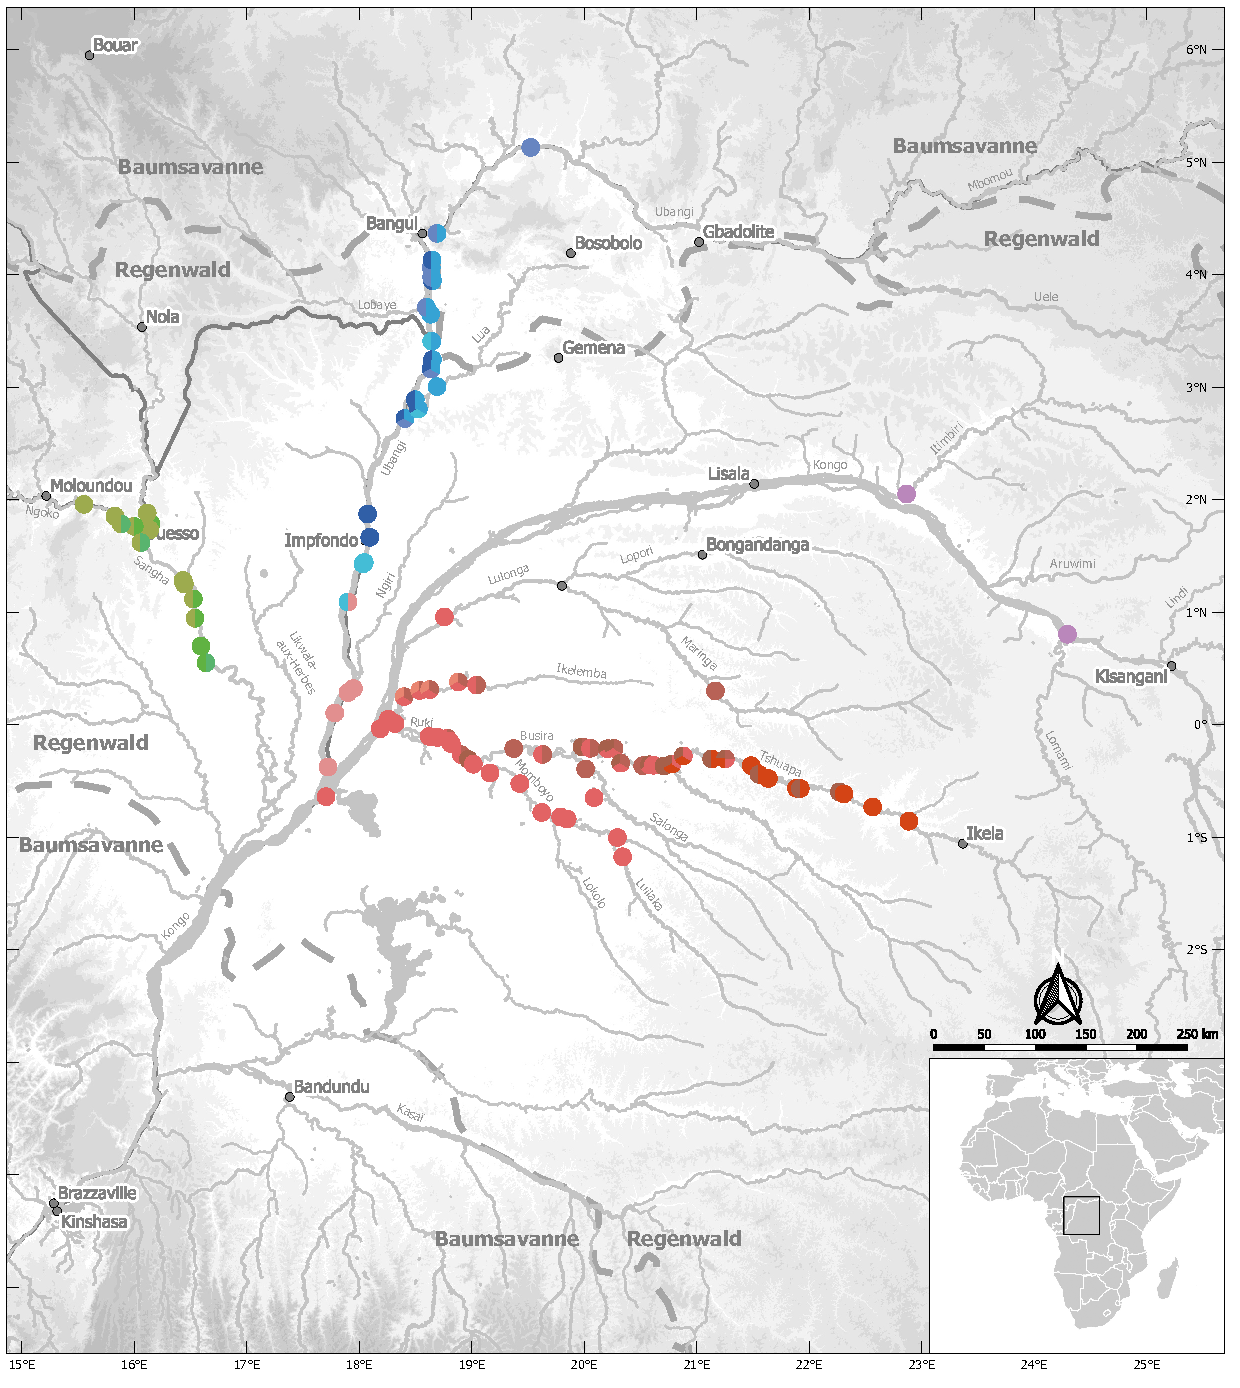
\includegraphics[width = \textwidth]{GIS/output/5-7_Zeitscheibe_LIA2_A4print-2.pdf}
		\vspace{2cm}
		\caption{Verbreitung}
		\label{fig:LIA2_Karte}
	\end{subfigure}
	\caption{Mittlere Phase der Späten Eisenzeit (17.--19. Jh. n. Chr.).}
	\label{fig:}
\end{figure*}
\addtocounter{figure}{-1}
\begin{figure*}[p]
	\begin{subfigure}[b]{\textwidth}
		\setcounter{subfigure}{1}
		\centering
		\includegraphics[width = \textwidth]{figs/Chronologiesystem_v3a_Zeitschiebe_LIA2.pdf}
		\caption{Chronologie}
		\label{fig:LIA2_Chronologie}
	\end{subfigure}
	\caption{Mittlere Phase der Späten Eisenzeit (17.--19. Jh. n. Chr.).}
	\label{fig:LIA2}
\end{figure*}

% Placing figure on an even/odd page [duplicate]
% https://tex.stackexchange.com/questions/55653/placing-figure-on-an-even-odd-page
\begin{figure*}[p]
	\centering
	\begin{subfigure}[b]{\textwidth}
		\centering
		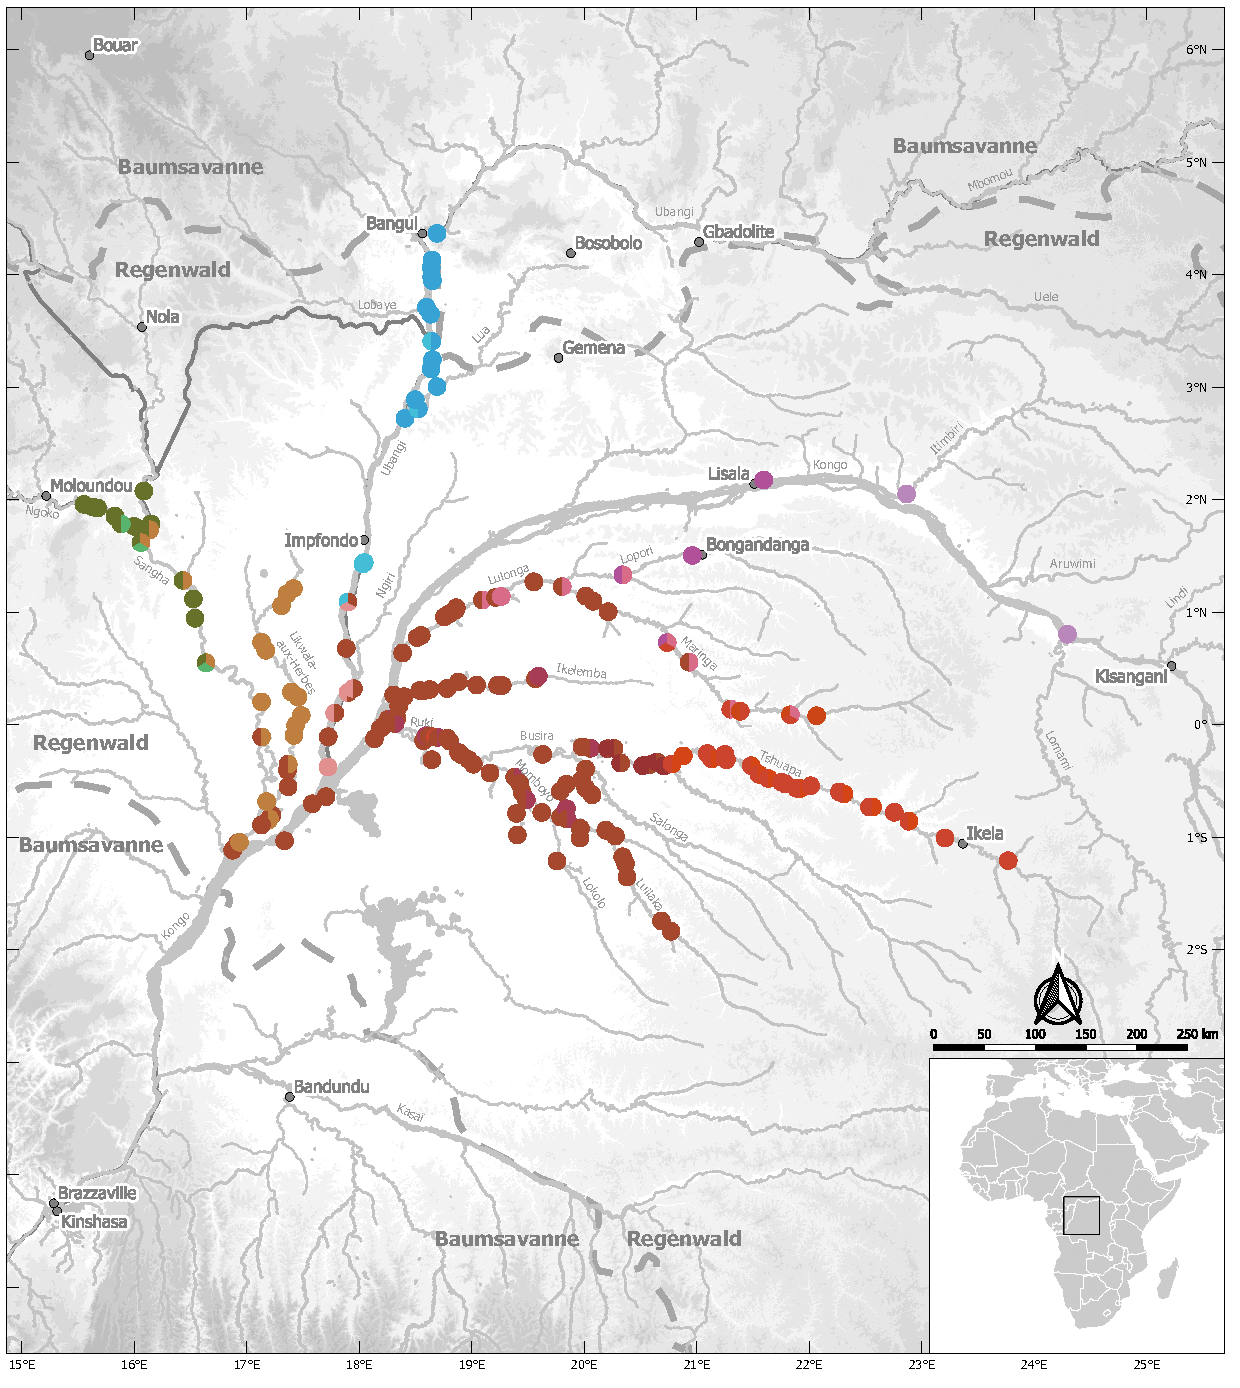
\includegraphics[width = \textwidth]{GIS/output/5-7_Zeitscheibe_LIA3_A4print-2.pdf}
		\vspace{2cm}
		\caption{Verbreitung}
		\label{fig:LIA3_Karte}
	\end{subfigure}
	\caption{Jüngere Phase der Späten Eisenzeit (20. Jh. n. Chr.).}
	\label{fig:}
\end{figure*}
\addtocounter{figure}{-1}
\begin{figure*}[p]
	\begin{subfigure}[b]{\textwidth}
		\setcounter{subfigure}{1}
		\centering
		\includegraphics[width = \textwidth]{figs/Chronologiesystem_v3a_Zeitschiebe_LIA3.pdf}
		\caption{Chronologie}
		\label{fig:LIA3_Chronologie}
	\end{subfigure}
	\caption{Jüngere Phase der Späten Eisenzeit (20. Jh. n. Chr.).}
	\label{fig:LIA3}
\end{figure*}

Im Norden und Westen des nordwestlichen Kongobeckens verstärkt sich der in den vorangegangen Jahrhunderten begonnene Trend zur Übernahme des Roulettedekors. Am mittleren Ubangi zeichnet sich die Motenge-Boma-Keramik (Kap.~\ref{sec:MTB-Gr}) durch einen massiven Einsatz von Schnitzroulettedekor aus, während die Pandama-Keramik (Kap.~\ref{sec:PDM-Gr}) am oberen Sangha und Ngoko vegetabilische Roulette sowie Ritzdekor aufweist. Die Rouletteverzierung bildet in diesen Regionen ab der mittleren Phase der Späten Eisenzeit die vorherrschende Verzierungstechnik.

Die ersten Kenntnisse aus ethno-historischen Quellen zur Töpfereitradition des Kongobeckens stammen aus dem ausgehenden 19. und beginnenden 20.~Jh.~n.~Chr. Von besonderer Bedeutung sind die Zusammenstellungen von \textcite{Coart.1907} der ethnografischen Bestände des \textit{Musée royal de l'Afrique centrale} in Tervuren bei Brüssel, in der sich unter anderem die Keramik der Botendo-Gruppe des Inneren Kongobeckens eindeutig identifizieren lässt \parencite[25 Anm.~12, 157]{Wotzka.1995}. Auch für die spitzbodigen, mutmaßlich in Bomongo am Ngiri produzierten Flaschen liegen Datierungsindizien aus historischen Zusammenhängen vor \parencite[167 Abb. III.11.1; Kap.~\ref{sec:SHG-LKW_Einzelfunde}]{OmasomboTshonda.2014}

\subsubsection*{Jüngere Phase der Späten Eisenzeit (20. Jh. n. Chr.)}

Die jüngere Phase der Späten Eisenzeit spiegelt die wissenschaftlich direkt untersuchten Töpfereitradtionen sowie noch in Benutzung vorgefundene Keramik des Kongobeckens wider. Im Zuge des \textit{River Reconnaissance Project} wurde in mehreren Dörfern die seinerzeit noch praktizierte Töpfereitechnik dokumentiert. Im Inneren Kongobecken wurde verstärkt die durch Treiben hergestellte Keramik des lokalen Töpfereizentrums in Ikenge am Ruki untersucht \parencites{Eggert.1980c}{Wotzka.1991}. Diese wird von Töpferinnen auf dem lokalen Markt sowie in der Provinzhauptstadt Mbandaka verhandelt \parencites[395f.;]{Eggert.1980c}{Eggert.1991}. Darüber hinaus wurde Töpferei noch in Liyolongo am Busira und Balinga-Bokonda am Tshuapa sowie Yopoko am Maringa beobachtet und untersucht \parencite[188, 196f.; Kap.~\ref{sec:ToepfereiEthnogr}]{Wotzka.1991}. Auch in diesen Orten wurden die Gefäße durch Treiben hergestellt, wobei an diesen Orten geflochtene Matten oder grobes Korbgeflecht als Unterlage genutzt wurden, eine Praxis die in Ikenge so nicht beobachtete wurde.

Im nordwestlichen Kongobecken wurde die Töpferei an vier Fundstellen beobachtet: in Boleko an der Mündung des Likwala-aux-Herbes wurde die Produktion von Gefäßen des Ebambe-Stils (Kap.~\ref{sec:EBA-Gr}) beobachtete, die ähnlich der Keramik des Inneren Kongobeckens durch Treiben hergestellt wurden. In Pikunda am mittleren Sangha und Mbati-Ngombe am mittleren Ubangi ließen sich in Aufbautechnik arbeitende Töpferinnen beobachten und im äußersten Norden, in Dama~I, Boduna und Sidi wurde die Herstellung in Abformtechnik dokumentiert (Abb.~\ref{fig:Keramikherstellung_Karte}). Während die Töpferei in Mbati-Ngombe und Dama~I jeweils spezifischen Stilen zugeordnet werden kann (Kap.~\ref{sec:DAM-Gr}--\ref{sec:MBN-Gr}), weisen die in Pikunda getöpferten Gefäße starke stilistische Ähnlichkeiten zur Keramik der Pandama-Gruppe (Kap.~\ref{sec:PDM-Gr}) auf, ohne ihr gänzlich zu entsprechen. Von der entlang des oberen Sangha und Ngoko beobachteten rezenten Mbenja-Keramik unterscheidet sie sich durch ihre ausschließliche Nutzung vegetabilischen Roulettes, wo bei der Mbenja-Keramik ausschließlich Schnitzroulette Verwendung findet. Die auf Herstellungsspuren untersuchten, der \textit{Ngoko-Tradition} zurechenbaren Gefäße der Stile Mandombe und Konda (Kap.~\ref{sec:Herstellung2_Toepferei}; Abb.~\ref{PIK87-1-2-3_1-3-7_Makrospuren}) deuten ebenfalls auf eine Herstellung in Aufbautechnik hin. Es kann daher als starke Hypothese gelten, dass die Keramik der \textit{Ngoko-Tradition} generell in dieser Technik hergestellt wurde und sich dadurch auch von der Töpferei des Inneren Kongobeckens unterscheidet. Die weiter stromab am unteren Sangha sowie dem Likwala-aux-Herbes beobachteten modernen Stile Epena (Kap.~\ref{sec:EPE-Gr}) und Mobaka (Kap.~\ref{sec:MKA-Gr}) sowie die bereits genannte Ebambe-Keramik entsprechen -- soweit untersucht -- in ihren \textit{Fabrics} sowie Hinweisen auf eine Herstellung durch Treiben der Keramik des Inneren Kongobeckens. Da sie auch stilistische Bezüge zur weiter östlich praktizierten Töpferei aufweisen, kann erwogen werden sie als Teil der von \textcite[222 Abb.~4, 224, 273]{Wotzka.1995} beschriebenen \textit{Äquator-Co-Tradition} anzusehen.

Am oberen Ubangi, im äußersten Norden des Arbeitsgebietes, fanden sich neben den Vertretern der bereits erwähnten Keramik aus Dama auch noch die Gefäße der Kpetene-Gruppe (Kap.~\ref{sec:KPT-Gr}), die stilistisch deutliche Unterschiede zueinander aufweisen. Etwas weiter stromab fand sich zudem noch ein gänzlich ohne Rouletteverzierung auskommender keramischer Stil, der nach der Haupstadt der Zentralafrikanischen Republik Bangui benannt wurde (Kap.~\ref{sec:BAN-Gr}). Diese ist insofern erwähnenswert, da alle anderen zeitgleichen Töpfereierzeugnisse der Region durchweg eine fast ausschließlich durch Roulettetechnik bestimmte Verzierungspraxis zeigen. Aus dem nordöstlichen Kongobecken liegen keine dezidierten Beschreibungen der rezenten Töpferei vor.

Die jüngere Phase der Späten Eisenzeit zeichnet sich durch eine Intensivierung der bereits in der vorangegangen Phase beobachteten Regionalisierung der keramischen Entwicklungen aus. Auch lassen sich durch die Verbindung von Beobachtungen der Töpferei an wenigen Plätzen in den entsprechenden Verbreitungsgebieten der Erzeugnisse die lokalen Distributionsnetze ablesen.